\documentclass[12pt,a4paper,oneside,pdftex]{report}
\usepackage[latin1]{inputenc}
\usepackage[OT1]{fontenc}
\usepackage[finnish,swedish,english]{babel}
\usepackage[square,sort&compress,numbers]{natbib}
\usepackage{eurosym} 
\usepackage{verbatim}
\usepackage{longtable}
\usepackage{subcaption}
\usepackage[medium]{titlesec}

\usepackage{amssymb}
\usepackage{amsmath}
\usepackage[ruled,linesnumbered]{algorithm2e}
% \usepackage[show]{notes}

% The TikZ package allows you to create professional technical figures.
% The learning curve is quite steep, but it is definitely worth it if 
% you wish to have really good-looking technical figures. 
\usepackage{tikz}
% You also need to specify which TikZ libraries you use
\usetikzlibrary{positioning}
\usetikzlibrary{calc}
\usetikzlibrary{arrows}
\usetikzlibrary{arrows.meta}
\usetikzlibrary{decorations.pathmorphing,decorations.markings}
\usetikzlibrary{shapes}
\usetikzlibrary{patterns}
\usepackage{todonotes}
\usepackage{amsthm}
\usepackage{booktabs}
\usepackage{multirow}


\DeclareMathOperator*{\src}{src}
\DeclareMathOperator*{\dest}{dest}
\DeclareMathOperator*{\sgn}{sgn}


\newcommand{\notimplies}{%
\mathrel{{\ooalign{\hidewidth$\not\phantom{=}$\hidewidth\cr$\implies$}}}}


\newcommand{\localintersect}{\cap_{l}}
\newcommand{\indegree}{d_{\text{in}}}
\newcommand{\outdegree}{d_{\text{out}}}

\newcommand{\mainNS}{{\sc main}\xspace}
\newcommand{\articleNS}{{\sc article}\xspace}
\newcommand{\helpNS}{{\sc help}\xspace}
\newcommand{\userNS}{{\sc user}\xspace}
\newcommand{\usertalkNS}{{\sc user talk}\xspace}
\newcommand{\usercontrib}{{\sc user-contrib}\xspace}
\newcommand{\wikirfa}{{\sc wiki-Rfa}\xspace}
\newcommand{\posPR}{$\text{PR}_{\text{pos}}$\xspace}
\newcommand{\posF}{$\text{F1}_{\text{pos}}$\xspace}
\newcommand{\negF}{$\text{F1}_{\text{neg}}$\xspace}
\newcommand{\macroF}{$\text{F1}_{\text{macro}}$\xspace}
\newcommand{\negPR}{$\text{PR}_{\text{neg}}$\xspace}
\newcommand{\aucnegPR}{AUC-\negPR}
\newcommand{\aucposPR}{AUC-\posPR}
\newcommand{\iterStatus}{{\sc iterative-status}\xspace}
\newcommand{\plusrightarrow}{\xrightarrow{+}}
\newcommand{\minusrightarrow}{\xrightarrow{-}}
\newcommand{\plusleftarrow}{\xleftarrow{+}}
\newcommand{\minusleftarrow}{\xleftarrow{-}}

% The aalto-thesis package provides typesetting instructions for the
% standard master's thesis parts (abstracts, front page, and so on)
% Load this package second-to-last, just before the hyperref package.
% Options that you can use: 
%   mydraft - renders the thesis in draft mode. 
%             Do not use for the final version. 
%   doublenumbering - [optional] number the first pages of the thesis
%                     with roman numerals (i, ii, iii, ...); and start
%                     arabic numbering (1, 2, 3, ...) only on the 
%                     first page of the first chapter
%   twoinstructors  - changes the title of instructors to plural form
%   twosupervisors  - changes the title of supervisors to plural form
\usepackage[mydraft]{aalto-thesis}
%\usepackage[mydraft,doublenumbering]{aalto-thesis}
%\usepackage{aalto-thesis}


% Hyperref
% ------------------------------------------------------------------
% Hyperref creates links from URLs, for references, and creates a
% TOC in the PDF file.
% This package must be the last one you include, because it has
% compatibility issues with many other packages and it fixes
% those issues when it is loaded.   
%\RequirePackage[pdftex]{hyperref}
\RequirePackage[pdfa]{hyperref}
% Setup hyperref so that links are clickable but do not look 
% different
\hypersetup{colorlinks=false,raiselinks=false,breaklinks=true}
\hypersetup{pdfborder={0 0 0}}
\hypersetup{bookmarksnumbered=true}
% The following line suggests the PDF reader that it should show the 
% first level of bookmarks opened in the hierarchical bookmark view. 
\hypersetup{bookmarksopen=true,bookmarksopenlevel=1}
% Hyperref can also set up the PDF metadata fields. These are
% set a bit later on, after the thesis setup.   
\usepackage{cleveref}

% Thesis setup
% ==================================================================
% Change these to fit your own thesis.
% \COMMAND always refers to the English version;
% \FCOMMAND refers to the Finnish version; and
% \SCOMMAND refers to the Swedish version.
% You may comment/remove those language variants that you do not use
% (but then you must not include the abstracts for that language)
% ------------------------------------------------------------------
% If you do not find the command for a text that is shown in the cover page or
% in the abstract texts, check the aalto-thesis.sty file and locate the text
% from there. 
% All the texts are configured in language-specific blocks (lots of commands
% that look like this: \renewcommand{\ATCITY}{Espoo}.
% You can just fix the texts there. Just remember to check all the language
% variants you use (they are all there in the same place). 
% ------------------------------------------------------------------
\newcommand{\TITLE}{Inferring Voting Networks in Online Elections}
\newcommand{\FTITLE}{��nestysverkkojen p��telm�t online-vaaleissa}
\newcommand{\STITLE}{Avsluta omr�stningsn�tverk i onlineval}
\newcommand{\SUBTITLE}{}
\newcommand{\FSUBTITLE}{}
\newcommand{\SSUBTITLE}{}
\newcommand{\DATE}{March 14, 2020}
\newcommand{\FDATE}{20. maaliskuuta 2020}
\newcommand{\SDATE}{Den 20 mars 2020}

% Supervisors and instructors
% ------------------------------------------------------------------
% Usually thesis have one supervisor and one advisor. Sometimes you
% may have two advisors and, in double degree
% programs, you may have two supervisors. 
% If you have two supervisors, write both names here, separate them with a 
% double-backslash (see below for an example)
% Also remember to add the package option ``twosupervisors'' or
% ``twoinstructors'' to the aalto-thesis package (aalto-thesis.sty
% file line 72), so that the titles are in plural.
% Example of one supervisor:
\newcommand{\SUPERVISOR}{Professor Aristides Gionis}
\newcommand{\FSUPERVISOR}{Professori Aristides Gionis}
\newcommand{\SSUPERVISOR}{Professor Aristides Gionis}
% Example of twosupervisors:
% \newcommand{\SUPERVISOR}{Professor Antti Yl�-J��ski\\
%   Professor Petra Perustieteilij�}
% \newcommand{\FSUPERVISOR}{Professori Antti Yl�-J��ski\\
%   Professori Petra Perustieteilij�}
% \newcommand{\SSUPERVISOR}{Professor Antti Yl�-J��ski\\
%   Professor Petra Perustieteilij�}

% If you have only one instructor, just write one name here
\newcommand{\INSTRUCTOR}{Blank M.Sc. (Tech.)}
\newcommand{\FINSTRUCTOR}{Diplomi-insin��ri Blank}
\newcommand{\SINSTRUCTOR}{Diplomingenj�r Blank}
% If you have two instructors, separate them with \\ to create linefeeds
% \newcommand{\INSTRUCTOR}{Oili Ohjaaja M.Sc. (Tech.)\\
%  Elli Opas M.Sc. (Tech)}
%\newcommand{\FINSTRUCTOR}{Diplomi-insin��ri Oili Ohjaaja\\
%  Diplomi-insin��ri Elli Opas}
%\newcommand{\SINSTRUCTOR}{Diplomingenj�r Oili Ohjaaja\\
%  Diplomingenj�r Elli Opas}

% If you have two supervisors, it is common to write the schools
% of the supervisors in the cover page. If the following command is defined,
% then the supervisor names shown here are printed in the cover page. Otherwise,
% the supervisor names defined above are used.
% \newcommand{\COVERSUPERVISOR}{Professor Antti Yl�-J��ski, Aalto University\\
%   Professor Petra Perustieteilij�, University of Helsinki}

% The same option is for the instructors, if you have multiple instructors.
% \newcommand{\COVERINSTRUCTOR}{Oili Ohjaaja M.Sc. (Tech.), Aalto University\\
%  Elli Opas M.Sc. (Tech), Aalto SCI}


% Other stuff
% ------------------------------------------------------------------
\newcommand{\PROFESSORSHIP}{Computer Science}
\newcommand{\FPROFESSORSHIP}{Tietotekniikka}
\newcommand{\SPROFESSORSHIP}{Datateknik}
% Professorship code is the same in all languages
\newcommand{\PROFCODE}{SCI3042}
\newcommand{\KEYWORDS}{signed networks, balance, status, elections, Wikipedia, 
  voting, graphs}
\newcommand{\FKEYWORDS}{Finnish Keywords}
\newcommand{\SKEYWORDS}{Swedish Keywords}
\newcommand{\LANGUAGE}{English}
\newcommand{\FLANGUAGE}{Englanti}
\newcommand{\SLANGUAGE}{Engelska}

% Author is the same for all languages
\newcommand{\AUTHOR}{Ananth Mahadevan}


% Currently the English versions are used for the PDF file metadata
% Set the PDF title
\hypersetup{pdftitle={\TITLE\ \SUBTITLE}}
% Set the PDF author
\hypersetup{pdfauthor={\AUTHOR}}
% Set the PDF keywords
\hypersetup{pdfkeywords={\KEYWORDS}}
% Set the PDF subject
\hypersetup{pdfsubject={Master's Thesis}}


% Layout settings
% ------------------------------------------------------------------

% When you write in English, you should use the standard LaTeX 
% paragraph formatting: paragraphs are indented, and there is no 
% space between paragraphs.
% When writing in Finnish, we often use no indentation in the
% beginning of the paragraph, and there is some space between the 
% paragraphs. 

% If you write your thesis Finnish, uncomment these lines; if 
% you write in English, leave these lines commented! 
% \setlength{\parindent}{0pt}
% \setlength{\parskip}{1ex}

% Use this to control how much space there is between each line of text.
% 1 is normal (no extra space), 1.3 is about one-half more space, and
% 1.6 is about double line spacing.  
% \linespread{1} % This is the default
% \linespread{1.3}

% Bibliography style
% acm style gives you a basic reference style. It works only with numbered
% references.
\bibliographystyle{acm}
% Plainnat is a plain style that works with both numbered and name citations.
% \bibliographystyle{plainnat}


% Extra hyphenation settings
% ------------------------------------------------------------------
% You can list here all the files that are not hyphenated correctly.
% You can provide many \hyphenation commands and/or separate each word
% with a space inside a single command. Put hyphens in the places where
% a word can be hyphenated.
% Note that (by default) LaTeX will not hyphenate words that already
% have a hyphen in them (for example, if you write ``structure-modification 
% operation'', the word structure-modification will never be hyphenated).
% You need a special package to hyphenate those words.
\hyphenation{di-gi-taa-li-sta yksi-suun-tai-sta}



% The preamble ends here, and the document begins. 
% Place all formatting commands and such before this line.
% ------------------------------------------------------------------
\begin{document}
% This command adds a PDF bookmark to the cover page. You may leave
% it out if you don't like it...
\pdfbookmark[0]{Cover page}{bookmark.0.cover}
% This command is defined in aalto-thesis.sty. It controls the page 
% numbering based on whether the doublenumbering option is specified
\startcoverpage

% Cover page
% ------------------------------------------------------------------
% Options: finnish, english, and swedish
% These control in which language the cover-page information is shown
\coverpage{english}


% Abstracts
% ------------------------------------------------------------------
% Include an abstract in the language that the thesis is written in,
% and if your native language is Finnish or Swedish, one in that language.

% Abstract in English
% ------------------------------------------------------------------
\thesisabstract{english}{
abstract}

% Abstract in Finnish
% ------------------------------------------------------------------
\thesisabstract{finnish}{
Finnish Abstract
}

% Abstract in Swedish
% ------------------------------------------------------------------
\thesisabstract{swedish}{
Swedish abstract}


% Acknowledgements
% ------------------------------------------------------------------
% Select the language you use in your acknowledgements
\selectlanguage{english}

% Uncomment this line if you wish acknoledgements to appear in the 
% table of contents
%\addcontentsline{toc}{chapter}{Acknowledgements}

% The star means that the chapter isn't numbered and does not 
% show up in the TOC
\chapter*{Acknowledgements}

% I wish to thank all students who use \LaTeX\ for formatting their theses,
% because theses formatted with \LaTeX\ are just so nice.

% Thank you, and keep up the good work!
\vskip 10mm

\noindent Espoo, \DATE
\vskip 5mm
\noindent\AUTHOR

% Acronyms
% ------------------------------------------------------------------
% Use \cleardoublepage so that IF two-sided printing is used 
% (which is not often for masters theses), then the pages will still
% start correctly on the right-hand side.
\cleardoublepage
% Example acronyms are placed in a separate file, acronyms.tex
% \addcontentsline{toc}{chapter}{Abbreviations and Acronyms}
\chapter*{Abbreviations and Acronyms}

% The longtable environment should break the table properly to multiple pages, 
% if needed

\noindent
\begin{longtable}{@{}p{0.25\textwidth}p{0.7\textwidth}@{}}
2k/4k/8k mode & COFDM operation modes \\
3GPP & 3rd Generation Partnership Project \\ 
ESP & Encapsulating Security Payload; An IPsec security protocol \\ 
FLUTE  & The File Delivery over Unidirectional Transport protocol \\ 
e.g.& for example (do not list here this kind of common acronymbs or abbreviations, but only those that are essential for understanding the content of your thesis. \\ 
note & Note also, that this list is not compulsory, and should be omitted if you have only few abbreviations

\end{longtable}


% Table of contents
% ------------------------------------------------------------------
\cleardoublepage
% This command adds a PDF bookmark that links to the contents.
% You can use \addcontentsline{} as well, but that also adds contents
% entry to the table of contents, which is kind of redundant.
% The text ``Contents'' is shown in the PDF bookmark. 
\pdfbookmark[0]{Contents}{bookmark.0.contents}
\tableofcontents

% List of tables
% ------------------------------------------------------------------
% You only need a list of tables for your thesis if you have very 
% many tables. If you do, uncomment the following two lines.
% \cleardoublepage
% \listoftables

% Table of figures
% ------------------------------------------------------------------
% You only need a list of figures for your thesis if you have very 
% many figures. If you do, uncomment the following two lines.
% \cleardoublepage
% \listoffigures

% The following label is used for counting the prelude pages
\label{pages-prelude}
\cleardoublepage

%%%%%%%%%%%%%%%%% The main content starts here %%%%%%%%%%%%%%%%%%%%%
% ------------------------------------------------------------------
% This command is defined in aalto-thesis.sty. It controls the page 
% numbering based on whether the doublenumbering option is specified
\startfirstchapter

% Add headings to pages (the chapter title is shown)
\pagestyle{headings}
% The contents of the thesis are separated to their own files.
% Edit the content in these files, rename them as necessary.

%------------------------------------------------------------------
\chapter{Introduction}



In recent years, researchers have become increasingly interested in understanding the behaviour of voters in social networks. Knowledge of the factors that motivate voters, for example, voting for bills in the United States Congress \cite{karimi2019multicongress} or electing administrators in Wikipedia \cite{jankowski-lorek2013MBSN,cabunducan2011voting,lee2012uncovering}, is of great importance in selecting successful policies or candidates. Voting is a classic problem and has been studied extensively in the fields of game theory and political science \cite{zou2015strategicDoodle,kearns2009behavioral,tal2015a}. More recently, there is a focus on using information from networks formed from the interaction of voters to model their behaviour. This provides an insight into these interactions and into the influence of certain individuals on voters within a community.

In many communities, decision making is carried out through votes.
In these voting sessions, voters indicate if they are for or against an agenda through their vote.
These votes can be represented as positive or negative links in a \textit{signed network}.
Analysing this network of voting yields various interesting insights.
For instance, using methods such as correlation clustering \cite{brito2020aBrazil,levorato2016brazilian,chiang2014prediction} on these signed networks reveals communities that vote similarly and have common ideologies. 
This provides us with a macroscopic perspective of election dynamics and voting blocks.

On the other hand, predicting the sign of future links in these signed networks gives us a local understanding of the nodes in the network \cite{leskovec2010predicting,leskovec2010signed,chiang2011exploiting}.
This task is called \textit{sign prediction} and translates into predicting future votes in the voting networks.
The methods to predict the sign of a link use social theories of balance and status.
For instance, balance theory states that a friend of an enemy is likely to be an enemy \cite{harary1953on}.
Therefore, if a user disagrees with a common neighbour who supports an agenda, then they are more likely to oppose that agenda. 
Similarly, status theory states that people interact on the basis or relative merit \cite{leskovec2010predicting}.
Hence, if you disregard someone who in turn disregards an agenda, then you are more likely to disregard that agenda.
These social theories provide a strong framework, using which we can predict future interactions betweens voters and an agenda within a community.
By quantifying agreement or respect in a particular community, we can understand the motivations and factors that affect an individual voter's decision.

The traditional sign prediction approaches are abstract and general, so that they can be applied to signed networks that may not be voting networks \cite{agrawal2013link,khodadadi2017sign,Shuang-Hong2012Friend}.
Therefore, they disregard the iterative and chronological nature in which voting usually happens.
Furthermore, these methods rely on features obtained from counting triangles or \textit{triads}, to encode the theories of balance and status.
Hence, they fail to incorporate larger effects of balance and status in a network.
Moreover, in cases where research does focus on sign prediction in voting networks, they heavily rely on non-voting features of the voters and agendas.
They utilize these features and build bespoke machine learning models that are task-specific and static \cite{karimi2019multicongress,jankowski-lorek2013MBSN}.

Firstly, in this thesis, we propose a method to extend conventional sign prediction for the task of \textit{independent vote prediction}.
For an independent voter, we define the \textit{voting neighbourhood} with respect to a graph and the previous voters in the session.
Then, we gather the features from several \textit{auxiliary graphs} that contain non-voting relationships between users.
Furthermore, we collect triadic information from the voting network and create a combined feature vector for a voter.
Therefore, we formulate a supervised machine learning problem to classify and predict the sign of a vote, using true sign of the votes as targets.
This \textit{graph combination model} can be trained with any general linear method using appropriate data processing techniques.

Secondly, we present a novel iterative framework that utilizes theories of balance and status in the \textit{local signed network} (LSN) of a voter to predict the sign of their vote.
The framework maintains and constantly updates a \textit{relationship graph}.
The edges of this graph capture interaction between voters such as agreement or concurrence.
The LSN is defined as the intersection of the relationship graph with the graph of the current voting session.
Then, we quantify how much the LSN complies with balance theory or status theory by utilizing the spectral decomposition or the \textit{agony} of the LSN respectively.
This allows us to predict the vote as the edge, that when added to the LSN, complies more with either balance or status theory.
Therefore, we create two models, namely an \textit{iterative balance model} and an \textit{iterative status model}.
These models are iterative as, once the voting is completed in a session, they update their relationship graph with the information from the session.
Therefore, these models can be bootstrapped to start with no prior information and improve over time.

Users in Wikipedia undergo a process called a \textit{Request for Adminship} (RfA), to gain administrative privileges.
Candidates are nominated and the RfA is a week long period in which any registered Wikipedia user can show their support for or opposition towards the candidate.
After the community finishes its discussions and voting towards the candidate, the result of the RfA is decided by a Bureaucrat (a special class of users).
Upon success, the candidate is granted administrative privileges, and upon failure, the candidate can appear for a renomination after a period of time.

We implement the models proposed to predict the votes in Wikipedia RfA elections.
The results show that the iterative models far out-perform the graph combination model at predicting votes.
We explore the consequences of the voting order on the overall performance of the iterative models.
Furthermore, we analyse the features of both models to understand how well the theories of balance and status represent votes in Wikipedia elections and possible scope for future work.

\section{Thesis Outline}
The rest of the thesis is organized in the following manner. Firstly, we discuss the background relating to signed graphs and hierarchy in directed networks in Chapter~\ref{chp:background}. Next, in Chapter~\ref{chp:vote-prediction} we describe the vote prediction problem and approaches to solving it. Chapter~\ref{chp:wikipedia} provides a comprehensive view of Wikipedia and the election process for administrators. In Chapter~\ref{chp:implementation} we explain the datasets used, construction of the model and evaluation criteria. After that, we report our findings in Chapter~\ref{chp:results} and discuss their implications. Finally, we conclude the thesis and present future work in Chapter~\ref{chp:conclusion}.


\chapter{Graph Theory}
\label{chp:graph-theory}
\todo[inline,backgroundcolor=red!25]{Change Chapter to Background and include signed link prediction theory here as well}
In this chapter, we will provide the fundamentals of the graph theory concepts required to understand the rest of the thesis. In Section~\ref{sec:prelim} we cover the basic definitions and terminologies used to describe different types of graphs. Then we define a signed graph and discuss its unique properties in Section~\ref{sec:signed-graphs}. We outline the social theories of balance and status in signed networks in \Cref{sec:balance-theory,sec:status-theory}.\todo{Add line for link prediction} Lastly, we explain techniques of finding hierarchies in directed networks and the concept of agony in Section~\ref{sec:hierarchy}.

\section{Preliminaries}
\label{sec:prelim}
In this section, we define the various types of graphs and their basic properties. The notation and terminologies used closely follow those used in Diestel~\cite{diestel1997graph}. Graphs are structures that describe relationships between entities. These entities are called \textit{vertices} and entities related to one another are joined by edges. The terms graph, vertices and edges can be used interchangeably with \textit{network}, \textit{nodes} and \textit{links} respectively.

Graphs can be classified broadly into two types based on whether the edges posses a direction. We now go on to define them in detail.
\subsection{Undirected Graphs}
An undirected graph is pair $G=(V,E)$, where $V$ is the set of vertices and $E$ is the set $E \subseteq \{ (u,v) \mid u,v \in V\}$ of unordered pairs of vertices called edges. In this thesis we will deal only with \textit{simple graphs}, i.e. no self loops, $(u,v)\in V \times V, ~ u\neq v$ and there is at most one edge between vertices $u$ and $v$. 

The number of the vertices in a graph is called the \textit{order} of the graph and is denoted by $n= |G|$. In turn, the \textit{size} of a graph is the number of edges denoted by $m = \|G\|$ or $m=|E|$. A vertex $u$ is \textit{adjacent} to $v$ if they are the end points of an edge, $(u,v) \in E$. All the vertices adjacent to a vertex $v$ is called the \textit{neighbourhood} of $v$ and is denoted by $N(v)$. The \textit{degree} of a vertex $v$ is the number of nodes adjacent to that vertex and is denoted by $d(v) = |N(v)|$. 

The edges of an undirected graph can also have an associated value. This value can indicate the distance or similarity between a pair of vertices. These values are called \textit{weights} and the corresponding graph is called a \textit{weighted undirected graph}. Therefore, a weighted graph is defined as a triple $G=(V,E,w)$, where $w:E \rightarrow \mathbb{R}^{+}$ is a function that maps an edge $e$ to a positive real weight $w(e)$. Now an \textit{unweighted graph} is simply a weighted graph where the function $w$ is defined as: if $e \in E$ then $w(e)=1$ else $w(e)=0$. The degree of a vertex $v$ in a weighted graph is the sum of the weights to all the neighbours of $v$ and is defined as $d(v) = \sum_{u\in N(v)}w((u,v))$. An example of a weighted undirected graph is shown in Figure~\ref{fig:weighted-undirected}. 
\begin{figure}[!ht]
    \centering
    \tikzset{
    position/.style args={#1:#2 from #3}{
        at=(#3.#1), anchor=#1+180, shift=(#1:#2)
    }
}

\begin{tikzpicture}

    \begin{scope}[every node/.style={circle,thick,draw}]
        \node (v1) at (0,0) {$v_1$};
        \node[below=1cm of v1] (v2) {$v_2$};
        \node[position=45:2cm from v2] (v3) {$v_3$};
        \node[position=150:2cm from v1] (v4) {$v_4$};
        \node[left=3cm of v2] (v5) {$v_5$};
        \node[position=45:1cm from v5] (v6) {$v_6$};
    \end{scope}

    \begin{scope}[>={Stealth[red]},
        every edge/.style={thick,draw},
        every node/.style={fill=white,circle}]
        % \draw (v4) -- (v1) -- (v3) -- (v2) -- (v1);
        \path (v1) edge (v2) 
            (v2) edge (v3)
            (v1) edge node[above] {$1$} (v3)
            (v1) edge (v4)
            (v5) edge (v6)
            ;
    \end{scope}
  \end{tikzpicture}
  
    \caption{An example of a weighted undirected graph}
    \label{fig:weighted-undirected}
\end{figure}


\subsection{Directed Graphs}
The main distinction regarding a \textit{directed graph} (or \textit{digraph}) is that the edges are ordered pairs, i.e.$(u,v) \neq (v,u)$. Therefore, a directed graph has a similar definition: a pair $G=(V,E)$, where $V$ is the set of vertices and $E$ is the set of \textit{ordered} pairs of vertices. Now given an edge $e=(u,v)$ we can define a source function $\src:E\rightarrow V$ such that $\src(e)=u$ and a destination function $d:E\rightarrow V$ where $\dest(e)=v$. These functions classify the vertices in an edge $e$ as either the source or the destination. In this thesis, we deal only with \textit{simple directed graphs}, i.e. no self-loops, and there can be at most one edge from $u$ to $v$. 

As the edges now have an inherent direction, we can define the \textit{successors} and \textit{predecessors} of a node $v$. A vertex $u$ is called the \textit{successor} of a node $v$ if there exists a directed edge from $v$ to $u$, therefore the set of successors for a vertex $v$ can be defined as $S(v) = \{u \mid (v,u) \in E\}$. A \textit{predecessor} of a node $v$ is a vertex $u$ such that there exists a directed edge from $u$ to $v$, the set of predecessors for a vertex $v$ can de defined as $P(v) = \{u \mid (u,v) \in E\}$. Now, a vertex $u$ that is either a successor or a predecessor of a vertex $v$ can be called a neighbour of the vertex $v$. Therefore, we define the \textit{neighbourhood} of a vertex $v$ as the set of vertices in the union of successors and predecessor, i.e. $N(v) = S(u) \cup P(v)$. This definition is also compatible with undirected graphs because if $(u,v) \in E$ then $(v,u) \in E$. 

Directed graphs can also have values associated with each directed edge called a \textit{weight}. A \textit{weighted directed graph} can be defined as a triple $G=(V,E,w)$, where the weight function $w:E \rightarrow \mathbb{R}^{+}$ maps each edge $e$ to a weight $w(e)$. The indegree of a vertex $v$ is defined as the sum of the edge weights from the predecessors of $v$ and is denoted as $\indegree(v) = \sum_{u \in P(v)} w((u,v))$. Similarly, the outdegree of a vertex $v$ is defined as the sum of the edge weights to the successors of $v$ and is denoted by $\outdegree(v) = \sum_{u \in S(v)}w((v,u))$.
Figure~\ref{fig:weighted-directed} shows an example of a weighted directed graph.

\begin{figure}[!ht]
    \centering
    \tikzset{
    position/.style args={#1:#2 from #3}{
        at=(#3.#1), anchor=#1+180, shift=(#1:#2)
    }
}

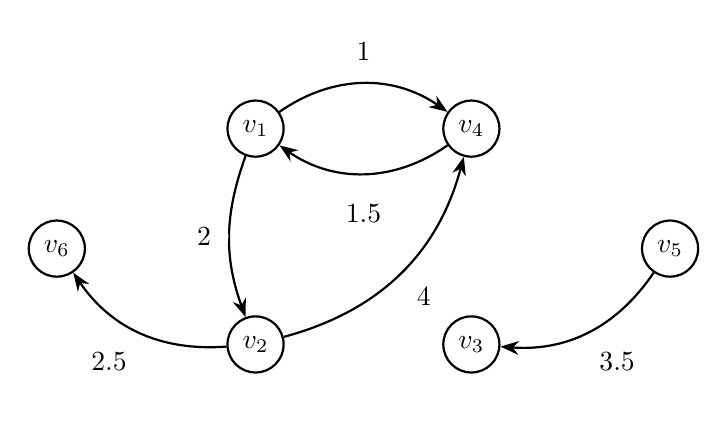
\begin{tikzpicture}

    \begin{scope}[every node/.style={circle,thick,draw}]
        \node (v1) at (0,0) {$v_1$};
        \node[below=2cm of v1] (v2) {$v_2$};
        \node[right=2cm of v2] (v3) {$v_3$};
        \node[above=2cm of v3] (v4) {$v_4$};
        \node[below right=1cm and 2cm of v4] (v5) {$v_5$};
        \node[below left=1cm and 2cm of v1] (v6) {$v_6$};
    \end{scope}

    \begin{scope}[>={Stealth[black]},
        every edge/.style={thick,draw},
        every node/.style={fill=white,circle}]
        % \draw (v4) -- (v1) -- (v3) -- (v2) -- (v1);
        \path[->] 
        (v1) edge[bend right=20] node[left] {$2$} (v2)
        (v2) edge[bend right=30] node[below right=1mm] {$4$} (v4)  
        (v1) edge[bend left=35] node[above=0.8mm] {$1$} (v4)
        (v4) edge[bend left=35] node[below=0.8mm] {$1.5$} (v1)
        (v5) edge[bend left=30] node[below right=1mm] {$3.5$} (v3)
        (v2) edge[bend left=30] node[below left=0.8mm and 0.8mm] {$2.5$} (v6)
        ;
    \end{scope}
  \end{tikzpicture}
  
    \caption{An example of a weighted directed graph}
    \label{fig:weighted-directed}
\end{figure}

\section{Signed Graphs}
\label{sec:signed-graphs}
The simple weighted graphs we have defined so far only have non-negative edge weights that can represent similarity or closeness. In the 1950s, social psychologists found it desirable to express liking, disliking or indifference in social interactions. This was formalized by Harary \cite{harary1953on} using graphs with weights $(-1,0,1)$. These graphs are therefore called \textit{signed graphs}, where a negative edge weight can denote dissimilarity between a pair of vertices. In this thesis we will use notations and terms similar to Gallier \cite{gallier2016spectral}, Kunegis et al.\ \cite{kunegis2010spectral}, Hou \cite{hou2005bounds} and Zaslavsky \cite{zaslavsky1982signed}.

A signed graph is a triple $G=(V,E,w)$, where $V$ is the set of vertices, $E$ is the set of pairs of vertices and the weight function $w:E \rightarrow \mathbb{R}$. The weight function now takes an edge $e$ and maps it to a signed weight $w(e)$. We can partition the edges into positive and negative edges, $E = E^{+}\cup E^{-}$, where $E^{+} = \{e \mid w(e)>0\}$ and $E^{-}=\{e \mid w(e)<0\}$. Similar to Zaslavsky \cite{zaslavsky1982signed}, we consider undirected signed graphs and directed signed graphs as distinct and separate entities. We can see some examples of signed graphs in Figure~\ref{fig:signed-graphs}.
\begin{figure}[!ht]
    \centering
    \begin{subfigure}{0.5\textwidth}
        \centering
        \tikzset{
    position/.style args={#1:#2 from #3}{
        at=(#3.#1), anchor=#1+180, shift=(#1:#2)
    }
}

\begin{tikzpicture}

    \begin{scope}[every node/.style={circle,thick,draw}]
        \node (v1) at (0,0) {$v_1$};
        \node[below=1cm of v1] (v2) {$v_2$};
        \node[position=45:2cm from v2] (v3) {$v_3$};
        \node[position=150:2cm from v1] (v4) {$v_4$};
        \node[left=3cm of v2] (v5) {$v_5$};
        \node[position=45:1.3cm from v5] (v6) {$v_6$};
    \end{scope}

    \begin{scope}[>={Stealth[red]},
        every edge/.style={thick,draw},
        every node/.style={fill=white,rectangle}]
        % \draw (v4) -- (v1) -- (v3) -- (v2) -- (v1);
        \path (v1) edge node[left] {$2$} (v2) 
            (v2) edge node[below right=0.05cm and 0.05cm] {$-1.5$} (v3)
            (v1) edge node[above=0.05cm] {$-1$} (v3)
            (v1) edge node[above right] {$4$} (v4)
            (v5) edge node[above left] {$-3$} (v6)
            ;
    \end{scope}
  \end{tikzpicture}
  
        \caption{A undirected signed graph}
        \label{fig:signed-undirected}
    \end{subfigure}

    \begin{subfigure}{0.5\textwidth}
        \centering
        \tikzset{
    position/.style args={#1:#2 from #3}{
        at=(#3.#1), anchor=#1+180, shift=(#1:#2)
    }
}

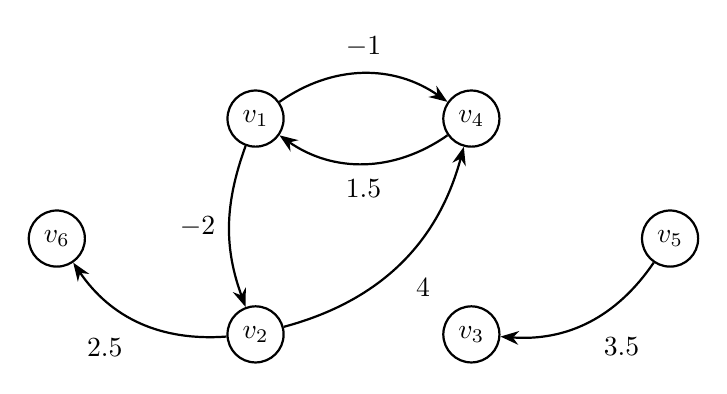
\begin{tikzpicture}

    \begin{scope}[every node/.style={circle,thick,draw}]
        \node (v1) at (0,0) {$v_1$};
        \node[below=2cm of v1] (v2) {$v_2$};
        \node[right=2cm of v2] (v3) {$v_3$};
        \node[above=2cm of v3] (v4) {$v_4$};
        \node[below right=1cm and 2cm of v4] (v5) {$v_5$};
        \node[below left=1cm and 2cm of v1] (v6) {$v_6$};
    \end{scope}

    \begin{scope}[>={Stealth[black]},
        every edge/.style={thick,draw},
        every node/.style={fill=white,rectangle}]
        % \draw (v4) -- (v1) -- (v3) -- (v2) -- (v1);
        \path[->] 
        (v1) edge[bend right=20] node[left=0.05cm] {$-2$} (v2)
        (v2) edge[bend right=30] node[below right=1mm] {$4$} (v4)  
        (v1) edge[bend left=35] node[above=0.8mm] {$-1$} (v4)
        (v4) edge[bend left=35] node[below=0.8mm] {$1.5$} (v1)
        (v5) edge[bend left=30] node[below right=1mm] {$3.5$} (v3)
        (v2) edge[bend left=30] node[below left=0.8mm and 0.8mm] {$2.5$} (v6)
        ;
    \end{scope}
  \end{tikzpicture}
  
        \caption{A directed signed graph}
        \label{fig:signed-directed graph}
    \end{subfigure}
    \caption{Examples of Signed Graphs}
    \label{fig:signed-graphs}
\end{figure}

We can now proceed to define a few more terms. The degree of a vertex $v$ is now the sum of the absolute edge weight of its neighbours, called the \textit{signed degree} and is defined as 
\[
    \overline{d}(v) = \sum_{u \in N(v)}|w((u,v))|
\] 
This can also be extended to \textit{signed indegree} and \textit{signed outdegree} denoted by $\overline{\indegree}(v)$ and $\overline{\outdegree}(v)$ and defined as
\[
    \overline{\indegree}(v)=\sum_{u \in P(v)}|w((u,v))|
\] 
\[
    \overline{\outdegree}(v)=\sum_{u \in S(v)}|w((v,u))|
\] 

We can create a $n \times n$ square weight matrix $W$, where each entry $w_{ij}$ is defined as 

\[ w_{ij} = 
\begin{cases}
    w((v_i,v_j)) & \text{if } (v_i,v_j) \in E \\
    0 & \text{if } (v_i,v_j) \notin E      
\end{cases}
\] 
The signed degree matrix $\overline{D}$ is a diagonal matrix consisting of the signed verted degrees, $\overline{D} = \text{diag}(\overline{d}(v_{1}),\dots,d(v_n))$. We can now define the \textit{signed Laplacian}, $\overline{L}$ as 
\[ \overline{L} = \overline{D} - W\]
The signed Laplacian along with results from spectral analysis of signed graphs \cite{hou2005bounds,kunegis2010spectral}, will be useful for balance theory of signed graphs. 

\subsection{Balance Theory}
\label{sec:balance-theory}


In the 1940s, Heider \cite{heider1946attitudes} proposed  that when there are either \textit{positive relations} (friendship, love, support) and \textit{negative relations} (enmity, hate, oppose) in a group, the  group tends towards \textit{balance}. Balance is the concept that all members aim to maintain consistency in the relations they share with other members of the group. In a group of three members this can be seen as having three positive relations or one positive and two negative relations. In Figure~\ref{fig:undirected-triads} the triads $B_1$ and $B_2$ are \textit{balanced} and mirror aphorisms such as "the friend of my friend is also a friend" and "the enemy of my enemy is a friend" respectively. Therefore, triads $B_3$ and $B_4$ can be called \textit{unbalanced} or \textit{imbalanced} that denotes the cognitive dissonance between the members of the triad. The dissonance can be understood by the counterintuitive nature of the phrase "the friend of my friend is my enemy" described by triad $B_3$.

Harary and Cartwright \cite{cartwright1956structural} generalized this notion of balance by using signed graphs. As these relations are typically symmetric, balance is usually defined for undirected signed graphs. This can been seen in Figure~\ref{fig:undirected-triads} where solid edges are positive and dashed edges are negative. Davies \cite{davis1963weakBalance} also offers an alternate definition of \textit{weak balance} where triads of type $B_2$ are considered to have lesser predictive utility as relationships of these type are less common in real-life social networks.

\begin{figure}[!ht]     
    \centering
    \tikzset{
    position/.style args={#1:#2 from #3}{
        at=(#3.#1), anchor=#1+180, shift=(#1:#2)
    }
}

\begin{tikzpicture}

    \begin{scope}[every node/.style={circle,thick,draw}]
        \node (v1) at (0,0) {};
        \node[position=-120:1cm from v1] (v2) {};
        \node[position=-60:1cm from v1] (v3) {};
        
        \node[right=2cm of v1] (v4) {};
        \node[position=-120:1cm from v4] (v5) {};
        \node[position=-60:1cm from v4] (v6) {};
        
        \node[right=2cm of v4] (v7) {};
        \node[position=-120:1cm from v7] (v8) {};
        \node[position=-60:1cm from v7] (v9) {};
        
        \node[right=2cm of v7] (v10) {};
        \node[position=-120:1cm from v10] (v11) {};
        \node[position=-60:1cm from v10] (v12) {};
        

    \end{scope}

    \begin{scope}[>={Stealth[red]},
        positive/.style={thick,draw},
        negative/.style={thick,dashed,draw},
        every node/.style={fill=white,circle}]
        % \draw (v4) -- (v1) -- (v3) -- (v2) -- (v1);
        \path 
        (v1) edge[positive] node[above left=0.1mm and 0.1mm] {$+$} (v2)
        (v1) edge[positive] node[above right=0.1mm and 0.1mm] {$+$} (v3) 
        (v3) edge[positive] node[below] {$+$} node[below=1cm] {$T_1$}  (v2)      
        ;
        \path 
        (v4) edge[negative] node[above left=0.1mm and 0.1mm] {$-$} (v5)
        (v4) edge[negative] node[above right=0.1mm and 0.1mm] {$-$} (v6) 
        (v6) edge[positive] node[below] {$+$} node[below=1cm] {$T_2$}  (v5)      
        ;
        \path 
        (v7) edge[positive] node[above left=0.1mm and 0.1mm] {$+$} (v8)
        (v7) edge[positive] node[above right=0.1mm and 0.1mm] {$+$} (v9) 
        (v9) edge[negative] node[below] {$-$} node[below=1cm] {$T_3$}  (v8)      
        ;
        \path 
        (v10) edge[negative] node[above left=0.1mm and 0.1mm] {$-$} (v11)
        (v10) edge[negative] node[above right=0.1mm and 0.1mm] {$-$} (v12) 
        (v12) edge[negative] node[below] {$-$} node[below=1cm] {$T_4$}  (v11)      
        ;
    \end{scope}
  \end{tikzpicture}
    
    \caption{Triads in undirected signed graphs. $B_1$ and $B_2$ are \textit{balanced} triads as they have even number of negative edges. $B_3$ and $B_4$ are \textit{unbalanced} as they have odd number of negative edges.}
    \label{fig:undirected-triads}
\end{figure}

The concept of balance can be generalized for an undirected signed graph $G=(V,E,w)$. The sign of a cycle $C$ in the signed graph $G$ is defined as the product of the edge weights $sgn(C)=\prod_{e\in C}w(e)$. A signed network $G$ is then said to be balanced if and only if all the sign of all cycles in network are positive. Therefore, every cycle in $G$ must have an even number of negative edges. This leads to result from Harary \cite{harary1953on} that states that if a graph $G$ is balanced, then there is a partition of the vertices $V = V_1 \cup V_2$ such that edges within the vertices of each set is positive and edges between the sets are negative. This means that we can have a bipartite graph when we delete the positive edges and negative edges span between the two sets of vertices. An example of a balanced signed graph is shown in Figure~\ref{fig:balanced-graph}. Here the partition of the vertex set is $V_1 = \{v_1,v_3,v_4,v_7,v_8\}$ and $V_2 = \{v_2,v_5,v_6,v_9\}$.

\begin{figure}[!ht]
    \centering
    \tikzset{
    position/.style args={#1:#2 from #3}{
        at=(#3.#1), anchor=#1+180, shift=(#1:#2)
    }
}

\begin{tikzpicture}

    \begin{scope}[every node/.style={circle,thick,draw}]
        \node (v1) at (0,0) {$v_1$};
        \node[position=-20:4cm from v1] (v2) {$v_2$};
        \node[position=-60:1.7cm from v2] (v5) {$v_5$};
        \node[position=55:2.3cm from v2] (v6) {$v_6$};
        \node[position=12:2.5cm from v2] (v9) {$v_9$};
        \node[position=-70:2cm from v1] (v3) {$v_3$};
        \node[position=-195:1.5cm from v3] (v4) {$v_4$};
        \node[position=225:2cm from v3] (v7) {$v_7$};
        \node[position=-90:2.4cm from v3] (v8) {$v_8$};
    \end{scope}

    % positive edges
    \begin{scope}[every edge/.style={thick,draw,blue},
        every node/.style={fill=white,circle}]
        % \draw (v4) -- (v1) -- (v3) -- (v2) -- (v1);
        \path 
        (v2) edge (v5) 
        (v5) edge (v9)
        (v2) edge (v6)
        (v6) edge (v5)
        (v2) edge (v9)      
        (v1) edge (v3)
        (v1) edge (v4)
        (v4) edge (v3)
        (v3) edge (v7)
        (v7) edge (v1)
        (v4) edge (v8)
        (v8) edge (v7)
        ;
    \end{scope}
    % negative edges
    \begin{scope}[every edge/.style={thick,draw,red,dashed},
        every node/.style={fill=white,circle}]
        % \draw (v4) -- (v1) -- (v3) -- (v2) -- (v1);
        \path 
        (v1) edge (v2)
        (v1) edge (v6)
        (v3) edge (v6)
        (v3) edge (v5)
        (v8) edge (v2)
        (v1) edge (v5)
        ;
    \end{scope}
  \end{tikzpicture}
  
    \caption{ A balanced signed graph. Solid blue edges are positive and dashed red edges are negative. Every cycle in this graph contains an even number of negative edges.}
    \label{fig:balanced-graph}
\end{figure}

The signed Laplacian matrix $\overline{L}$ of a signed graph $G$ is always positive-semidefinite and $\overline{L}$ is positive-definite iff $G$ is \textit{unbalanced} \cite{kunegis2010spectral,hou2005bounds,zaslavsky1982signed}. If the smallest eigenvalue of a graph $G$ is denoted by $\lambda_{1}(G)$, then $G$ is balanced iff $\lambda_{1}(G)=0$. Hou \cite{hou2005bounds} provides bounds on the value of $\lambda_{1}(G)$ and Li et al.\ \cite{li2016note} show that $\lambda_{1}(G)$ can be used as a measure of how far the signed graph $G$ is from being balanced.

\subsection{Status Theory}
\label{sec:status-theory}
Guha et al.\ \cite{guha2004propagation} mention implicitly that a signed edge from $u$ to $v$ can be interpreted in a asymmetric manner different from "friend" or "enemy". Leskovec et al.\ \cite{leskovec2010signed,leskovec2010predicting} introduce the concept of \textit{status} to contextualize directed singed edges. A positive edge $u \plusrightarrow v$ indicates that $v$ has a higher status than $u$ and a negative edge $u \minusrightarrow v$ means that $v$ has a lower status than $u$. This concept of relative status can be propagated transitively along multiple steps which might lead to contradictions with balance theory \cite{leskovec2010signed}.

Given three vertices $v_1,v_2$ and $v_3$, the presence of an edge $v_1 \plusrightarrow v_2$ indicates that $v_1$ thinks $v_2$ has higher status, the edge $v_2 \plusrightarrow v_3$ indicates that $v_2$ thinks $v_3$ has higher status. Now we wish to to close this triad with an edge from $v_3$ to $v_1$. Status theory would say that through transitivity $v_1$ has lower status than $v_3$, therefore the prediction is $v_3 \minusrightarrow v_1$. Whereas, in balance theory we would predict a positive edge $v_3 \plusrightarrow v_1$ to make the cycle have even number of negative edges. This example can be seen in triads $S_1$ and $S_2$ shown in Figure~\ref{fig:status-triads}.

There are also cases when status theory is ambivalent to the edge that closes a triad. Consider the example when we have the edges $v_1 \plusrightarrow v_2$ and $v_2 \minusrightarrow v_3$. If we were to indicate the status of a vertex $v$ using the function $\sigma(v)$, then the edges describe the following : $\sigma(v_2)>s(v_1) $ and $\sigma(v_2)>\sigma(v_3)$. Therefore, we have no knowledge of the relative difference in status between the vertices $v_1$ and $v_3$. Hence, both edges $v_3 \plusrightarrow v_1$ ($\sigma(v_3) > \sigma(v_1)$) and $v_3 \minusrightarrow v_1$ ($\sigma(v_1) > \sigma(v_3)$) are equally valid for status theory. Balance theory on the other hand can only predict $v_3 \minusrightarrow v_1$ to keep the triad balanced. This case is shown in Figure~\ref{fig:status-triads} as triads $S_3$ and $S_4$.

\begin{figure}[!ht] 
    \centering
    \tikzset{
    position/.style args={#1:#2 from #3}{
        at=(#3.#1), anchor=#1+180, shift=(#1:#2)
    }
}

\begin{tikzpicture}

    \begin{scope}[every node/.style={circle,thick,draw}]
        \node (v2) at (0,0) {$v_2$};
        \node[position=-120:1cm from v2] (v1) {$v_1$};
        \node[position=-60:1cm from v2] (v3) {$v_3$};
        
        \node[right=2.5cm of v2] (v5) {$v_2$};
        \node[position=-120:1cm from v5] (v4) {$v_1$};
        \node[position=-60:1cm from v5] (v6) {$v_3$};
        
        \node[right=2.5cm of v5] (v8) {$v_2$};
        \node[position=-120:1cm from v8] (v7) {$v_1$};
        \node[position=-60:1cm from v8] (v9) {$v_3$};
        
        \node[right=2.5cm of v8] (v11) {$v_2$};
        \node[position=-120:1cm from v11] (v10) {$v_1$};
        \node[position=-60:1cm from v11] (v12) {$v_3$};
        

    \end{scope}

    \begin{scope}[>={Stealth[black]},
        positive/.style={thick,draw,->},
        negative/.style={thick,dashed,draw,->},
        every node/.style={fill=white,circle}]
        % \draw (v4) -- (v1) -- (v3) -- (v2) -- (v1);
        \path 
        (v1) edge[positive] node[above left=0.1mm and 0.1mm] {$+$} (v2)
        (v2) edge[positive] node[above right=0.1mm and 0.1mm] {$+$} (v3) 
        (v3) edge[positive] node[below] {$+$} node[below=1cm] {$S_1$}  (v1)      
        ;
        \path 
        (v4) edge[positive] node[above left=0.1mm and 0.1mm] {$+$} (v5)
        (v5) edge[positive] node[above right=0.1mm and 0.1mm] {$+$} (v6) 
        (v6) edge[negative] node[below] {$-$} node[below=1cm] {$S_2$}  (v4)      
        ;
        \path 
        (v7) edge[positive] node[above left=0.1mm and 0.1mm] {$+$} (v8)
        (v8) edge[negative] node[above right=0.1mm and 0.1mm] {$-$} (v9) 
        (v9) edge[negative] node[below] {$-$} node[below=1cm] {$S_3$}  (v7)      
        ;
        \path 
        (v10) edge[positive] node[above left=0.1mm and 0.1mm] {$+$} (v11)
        (v11) edge[negative] node[above right=0.1mm and 0.1mm] {$-$} (v12) 
        (v12) edge[positive] node[below] {$+$} node[below=1cm] {$S_4$}  (v10)      
        ;
    \end{scope}
  \end{tikzpicture}
  
    \caption{Triads in directed signed graphs. Triads $S_2,S_3$ and $S_4$ are compliant with status theory. Only triads $S_1$ and $S_3$ are compliant with balance theory.}
    \label{fig:status-triads}
\end{figure}

Each positive link inwards ($\indegree^{+}(v)$) and negative link outwards ($\outdegree^{-}(v)$) increases status. Each positive link outwards ($\outdegree^{+}(v)$) and negative link inwards ($\indegree^{-}(v)$) decreases status. Therefore, $\sigma(v) = \indegree^{+}(v) + \outdegree^{-}(v) - \outdegree^{+}(v)- \indegree^{-}(v)$ is a heuristic for the status of a node \cite{leskovec2010predicting}. An interesting fact is that the edge $u \minusrightarrow v$ can be converted into positive edge in the opposite direction $u \plusleftarrow v$. This fact reduces the number of unique triads that can be formed using status theory and will be used in edge prediction tasks that will be discussed in coming chapters.

\section{Hierarchy in directed networks}
\label{sec:hierarchy}
Hierarchies exist in all social structures, from the explicit levels found in nature such as the food chain or organizational structures in businesses to more implicit stratification that occurs on social media or online networks. A common method to represent such hierarchies is through a tree, for example, the chain of command in the military or within governments. Trees have well defined levels and a single person at the top. If we generalize this structural concept then we get a \textit{Directed Acyclic Graph} (DAG) which represents a partial ordering set. DAGs have perfect hierarchy while structures such as cycles tend to have no hierarchy. Other directed graphs occur somewhere between these two extremes.

Gupte et al.\ \cite{gupte2011finding} provide a method to discern the levels of stratification present in a given directed network when no prior information of the hierarchy exists. They define a measure of the hierarchy of a given directed network $G$ as $h(G)$ along with a polynomial algorithm to find the largest hierarchy in that network. They define a concept of \textit{social agony} which posits that agony is present when a person having a higher rank in network interacts with a person who has a lower rank. Therefore, if we define the rank of a node in graph $G$ as the function $r:V \rightarrow \mathbb{N}$, then a directed edge $u \rightarrow v$ causes agony when $r(u)\geq r(v)$. The agony for the edge can be quantified as $\max(r(u)-r(v)+1,0)$. The agony of the graph $G$ wrt to rank function $r$ is defined as 
\[A(G,r) =  \sum_{(u,v)\in E} \max(r(u)-r(v)+1,0)\]
As nodes in a graph tend to minimize the overall agony, the agony of a network $G$ is the smallest possible agony over all possible ranking for $r$, $A(G) = \min_{r\in \text{Rankings}}A(G,r)$. The hierarchy of a given network $G$, denoted by $h(G)$ can now be expressed in terms of the agony of the network, $h(G)=1-\frac{1}{m}A(G)$, where $m$ is the number of edges. We can see examples of hierarchy in unweighted directed graph in Figure~\ref{fig:hierarchy}.

 
\begin{figure}[!ht]
    \centering
    \begin{subfigure}[t]{0.5\textwidth}
        \centering
        \tikzset{
    position/.style args={#1:#2 from #3}{
        at=(#3.#1), anchor=#1+180, shift=(#1:#2)
    }
}

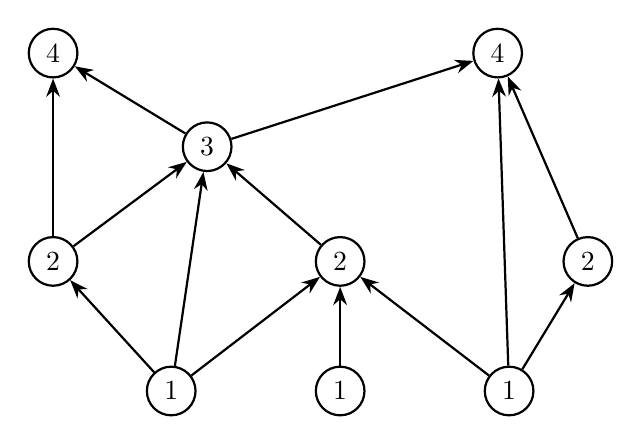
\begin{tikzpicture}

    \begin{scope}[every node/.style={circle,thick,draw}]
        \node (v1) at (0,0) {$1$};
        \node[right=1.5cm of v1] (v2) {$1$};
        \node[right=1.5cm of v2] (v3) {$1$};
        \node[above=1cm of v2] (v5) {$2$};
        \node[left=3cm of v5] (v4) {$2$};
        \node[right=2.5cm of v5] (v6) {$2$};
        \node[above right=1cm and 1.5cm of v4] (v7) {$3$};
        \node[above=2cm of v4] (v8) {$4$};
        \node[right=5cm of v8] (v9) {$4$};
    \end{scope}

    \begin{scope}[>={Stealth[black]},
        every edge/.style={thick,draw,->},
        every node/.style={fill=white,circle}]
        % \draw (v4) -- (v1) -- (v3) -- (v2) -- (v1);
        \path 
        (v1) edge (v4)
        (v1) edge (v7)
        (v1) edge (v5)
        (v2) edge (v5)
        (v3) edge (v5)
        (v3) edge (v6)
        (v3) edge (v9)
        (v4) edge (v7)
        (v4) edge (v8)
        (v5) edge (v7)
        (v6) edge (v9)
        (v7) edge (v8)
        (v7) edge (v9)

        ;
    \end{scope}
  \end{tikzpicture}
  
        \caption{DAG has perfect hierarchy, $h(G)=1$ and agony of each edge is 0}
        \label{fig:dag}
    \end{subfigure}

    \begin{subfigure}[t]{0.49\textwidth}
        \centering
        \tikzset{
    position/.style args={#1:#2 from #3}{
        at=(#3.#1), anchor=#1+180, shift=(#1:#2)
    }
}

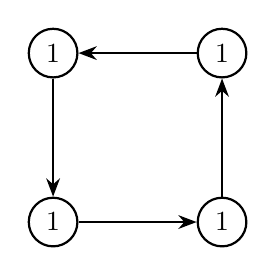
\begin{tikzpicture}

    \begin{scope}[every node/.style={circle,thick,draw}]
        \node (v1) at (0,0) {$1$};
        \node[right=1.5cm of v1] (v2) {$1$};
        \node[above=1.5cm of v2] (v3) {$1$};
        \node[left=1.5cm of v3] (v4) {$1$};

    \end{scope}

    \begin{scope}[>={Stealth[black]},
        every edge/.style={thick,draw,->},
        every node/.style={fill=white,circle}]
        % \draw (v4) -- (v1) -- (v3) -- (v2) -- (v1);
        \path 
        (v1) edge (v2)
        (v2) edge (v3)
        (v3) edge (v4)
        (v4) edge (v1)

        ;
    \end{scope}
  \end{tikzpicture}
  
        \caption{Cycle has no hierarchy, $h(G)=0$ and each edge has agony of 1}
        \label{fig:cycle}
    \end{subfigure}
    \begin{subfigure}[t]{0.49\textwidth}
        \centering
        \tikzset{
    position/.style args={#1:#2 from #3}{
        at=(#3.#1), anchor=#1+180, shift=(#1:#2)
    }
}

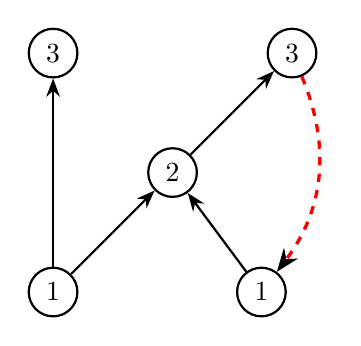
\begin{tikzpicture}

    \begin{scope}[every node/.style={circle,thick,draw}]
        \node (v1) at (0,0) {$1$};
        \node[right=2cm of v1] (v2) {$1$};
        \node[above right=1.5cm of v1] (v3) {$2$};
        \node[above left = 1.5cm of v3] (v4) {$3$};
        \node[above right=1.5cm of v3] (v5) {$3$};
    \end{scope}

    \begin{scope}[>={Stealth[black]},
        every edge/.style={thick,draw,->},
        back/.style ={very thick,dashed,red,->},
        every node/.style={fill=white,circle}]
        % \draw (v4) -- (v1) -- (v3) -- (v2) -- (v1);
        \path 
        (v1) edge (v3)
        (v1) edge (v4)
        (v2) edge (v3)
        (v3) edge (v5)
        (v5) edge[back,bend left] (v2)
        ;
    \end{scope}
  \end{tikzpicture}
  
        \caption{Graph with some hierarchy $h(G)=\frac{2}{5}$. Red dashed edge has agony of 3 and solid black edges have 0 agony.  }
        \label{fig:some-hierarchy}
    \end{subfigure}
    \caption{Examples of hierarchy in unweighted directed graphs. Numbers inside nodes indicate the rank of vertex.}
    \label{fig:hierarchy} 
\end{figure}

Therefore, finding a ranking of the nodes that minimizes the agony of the network gives us the optimal hierarchy present in that network. Gupte et al.\ \cite{gupte2011finding} and Tatti \cite{tatti2014faster} present a polynomial algorithm that can solve the dual of the agony minimization problem to obtain the optimal ranking $r$ for unweighted graphs. Tatti \cite{tatti2017tiers} provides an alternate approach using a capacitated circulation solver that can handle weighted digraphs as well as additional cardinality constraints. These algorithms allows us to find the levels of hierarchy present in any given directed social network and analyse the interaction between members belonging to different strata in that community.

We will explain in future chapters how hierarchies in social network is intrinsically linked to the theory of status in directed signed networks. We show one can use the concept of agony of a directed signed graph $G$ to quantify the violation to status theory and use it as a metric to predict an unknown signed edge.

\section{Link and Sign Prediction}
\label{sec:link-prediction}
The \textit{link prediction problem} is defined by Liben-Nowell and Kleinberg \cite{liben-nowell2007the} as inferring possible future edges between vertices in a social network. The datasets used was split into training edges and testing edges which had a common core set of vertices. They showed that topological features such as number of common neighbours and Katz's centrality index can be used in a unsupervised setting to accurately predict edges.

Leskovec et al.\ \cite{leskovec2010predicting} extended the link prediction problem to signed networks. They also introduced the problem of \textit{edge sign prediction}: predict the sign of a given edge $(u,v)$ using the existing signed network $G$. A supervised model for the task is proposed that uses network features such as indegree and outdegree of a node along with \textit{triad} features. The edge nodes $u$ and $v$ and a common neighbour $w$ form a triad. The directed edge between $(u,w)$ and $(w,u)$ can be either forward or backwards and each edge is either positive or negative. Therefore there are 16 possible triad types for a given neighbour $w$. They analyse these triadic features from the trained model and show how they relate to balance and status theory. For the link prediction problem, the information from the negative edges in the signed network offers improvement in the overall accuracy of the model. This seminal paper inspired many more approaches to solving these problems for signed graphs.   

Matrix factorization and latent space approaches facilitate link prediction and sign prediction tasks for multiple edges simultaneously in a signed network \cite{agrawal2013link,hsieh2012low,gu2019link}. Supervised algorithms for both tasks can be improved using additional node features such as inverse square metric \cite{ahmadalinezhad2018sign} or node rankings \cite{shahriari2014ranking}. Models that use graph motifs \cite{Liu2019LinkPrediction,khodadadi2017sign} generalize the concept of triadic feature for link and sign prediction. Chiang et al.\ generalize balance theory for longer cycles and use it as features to improve link prediction \cite{chiang2011exploiting}. Tang et al.\ \cite{Jiliang2015Negative} discuss the importance of predicting negative links and highlight methods to overcome the inherent imbalance present in signed network datasets. Cesa et al.\ \cite{cesa2012correlation} and Chiang et al.\ \cite{chiang2014prediction} utilize clustering techniques to solve sign prediction and link prediction respectively. Shuang et al.\ \cite{Shuang-Hong2012Friend}  and Karimi et al.\ \cite{karimi2019multicongress} create bespoke models incorporating user behaviour and political party affiliation respectively to predict the sign of edges present in the signed networks.




\chapter{Vote Prediction}
\label{chp:vote-prediction}
In this chapter, we cover the main motivation behind predicting the vote of an individual voter and present the methods that can be used to solve this task. We discuss the contrast in perspectives that is present when predicting the result compared to predicting a vote in Section~\ref{sec:result-vs-vote}. Next, we explain the link prediction problem in signed networks and the existing approaches as well as limitations to predicting votes in Section~\ref{sec:link-prediction}. In Section~\ref{sec:linear-combination-theory}, we describe a supervised machine learning framework that can use graphs from voting and non-voting features to predict a vote. Lastly, we present our novel approach of constructing a signed graph from neighbours of the current voter and previous votes and using balance and status theory to predict the vote in Section~\ref{sec:local-signed-network}. 


\section{Result versus Vote Prediction}
\label{sec:result-vs-vote}
In this thesis, we are interested in the voting behaviour for a collective action. In such cases, members of a community come together as \textit{voters} to decide on a particular \textit{candidate} item during a \textit{session}. In a government parliament  the voters are the elected members of the parliament and the candidate is usually a bill or policy matter. When it is promotion within a political party or an online community such as Wikipedia, the members vote on a candidate who has been nominated for the position. In all these cases we have two levels of decisions being made. The first the individual decisions that a voter makes with regard to the candidate. The second is the final decision that the group arrives to after everyone has voted. We refer to task of predicting the former as \textit{vote prediction} and the latter as \textit{result prediction}. 

Result prediction provides a macro level perspective of the incentives of a community. We can create models based on the characteristics of a candidate to predict the result of a collective action. This will lead to understanding on a communal level of what features are preferred and if there are voting blocks formed within the members based on the type of candidate. This translates to practical examples such as party level dynamics in a parliament, the topic of a bill or the credentials of a nominee \cite{burke2008mopping,yano2012textual,yogatama-etal-2011-predicting}. 

On the other hand, when we focus on the vote prediction problem, we get a deeper understanding of the dynamics between voters and the candidate. In fields such as game theory, this is well studied using frameworks such as \textit{strategic voting models} and \textit{momentum} \cite{meir2020strategic,zou2015strategicDoodle,ali2006a,banerjee1992simple}. These models are more theoretical and are studied under synthetic conditions. Nevertheless, they still provide a foundation on which we can construct practical models that can utilize additional external features. One such popular approach is using textual information from bills, speeches and legislature to predict votes of politicians in parliament \cite{budhwar2018predicting,gerrish2011predicting}. The next important step is to represent the voting data as networks and leveraging network features to understand and predict voter behaviour \cite{tal2015a,brito2020aBrazil,kearns2009behavioral,derr2018congressional,arinik2017signed}.

\section{Voting and Signed networks}
Votes by nature express a positive or negative relationship between a \textit{voter} and a \textit{candidate}. Therefore, \textit{signed graphs} provide an intuitive way to structurally represent the voting pattern of members in a community. These signed voting networks can be used to develop models to solve the task of vote prediction and analyse voter behaviour.

Correlation clustering and community detection of signed voting graphs can discover trends and vote blocks in communities \cite{brito2020aBrazil,arinik2017signed}. Analysing the networks using social theories of balance and status provides knowledge of voter behaviour and features for prediction methods \cite{levorato2016brazilian,derr2018congressional}. The vote prediction task can be broken down into two subtasks which are analogous to link and sign prediction in signed networks. 

The first subtask is to predict who will vote next given a candidate $c$ and a set of previous votes. This subtask is similar to link prediction in a signed network where we aim to predict possible future edges of the type $(v,c)$. The complexity subtask depends on the format of voting that takes place. If there is a known voting order, such as in roll call in parliamentary proceedings or explicit timestamps then it is essentially solved. If the voting occurs simultaneously, the subtask can be reduced to predicting the possible subset of members who will vote in a given session. When the voting is iterative and there is no known underlying process of who votes next, then a separate model might be required to infer the voting sequence. This case can be combinatorially hard as we would need to find the correct ordering of votes in a session.

The second subtask is to predict how a voter $v$ will vote for a candidate $c$ given the previous votes in the session. This task translates into predicting the sign of an edge $(v,c)$ in the current session. We call this subtask the \textit{independent vote prediction} problem. It is independent in nature are we are only interested in the decision of the voter $v$ assuming that we have complete prior knowledge of how the previous votes have been cast. This problem can be framed as a supervised learning task, using features of the interaction between the current voter $v$, previous voters $U$ and the candidate $c$ to predict the sign of the edge $(v,c)$. We can utilize theories of balance and status in signed networks to create models similar to those by Karimi et al. \cite{karimi2019multicongress} and Jankowski-Lorek et al. \cite{jankowski-lorek2013MBSN} to predict voter behaviour.

\iffalse
\todo[inline]{Are the IC paras neccessary?}
Information cascades are widely studied in epidemiology where we model the spread of a contagion through infections of neighbours and the halting using a rate of recovery. Collective voting in a network can be similarly modelled as a sequence of votes spreading through a network and naturally ending when a final decision has been taken. Using an \textit{independent cascade} model we can separate the spread of information in a network into two logical problems.

The first, is a which node will be affected next. This is equivalent to knowing which node will get infected in a contagion model or which person will be next to vote in a voter model. In contagions spread this is probabilistic hence can be easily modelled. This is different for voting models as some cases might have a fixed voting order while others may not. In the cases we have a known voting order such as the roll call for voting in parliament or timestamps in promotions of Wikipedia administrators, the problem is intrinsically solved. We have mentioned other models above, that can handle cases where there is either no known order or voting happens in a non-sequential manner. 

The second problem, is how will the node will react. In the context of a contagion model, this translates to whether the now infected node becomes sick or not. This is usually a known feature of a given contagion and hence is not critical to a contagion model. In a voter mode, this problem is determining how an individual voter will cast their vote given the information of who have already cast their vote. We call this problem the \textit{independent vote prediction} problem as it considers each voter in the chain as an independent actor and only aims to predict how that particular individual would vote. In solving this problem we can gain insights into the motivations and behaviour of voters. 

The problem of independent vote prediction is studied in Karimi et al. \cite{karimi2019multicongress} and Jankowski-Lorek et al.\cite{jankowski-lorek2013MBSN}. They propose models that incorporate network information, textual data, signed graph features to predict the voting behaviour. Although their models achieve a high predictive accuracy in their respective tasks, they are quite tasks specific and cannot easily be extended to other settings. In contrast, we focus on using general signed network features of balance and status to create a model to predict the votes. 

\fi

\section{Linear Combination of Graphs}
\label{sec:linear-combination-theory}

In this section we explain how the approaches outlined in Section~\ref{sec:link-prediction} can be applied to solve the \textit{independent vote prediction} problem. As discussed previously, the \textit{edge sign prediction} task in signed network is analogous to vote prediction. The models proposed by Leskovec et al. \cite{leskovec2010predicting} can be used to predict the sign of the edge $(v,c)$. Voting in a community takes place across many sessions in a chronological manner. Therefore, we must partition the training and testing datasets to avoid data leakage. We propose the following framework to gather features using a linear combination of the voting history and several auxiliary graphs.

We denote the directed signed graph for the current voting session as $S=(V_S,E_S)$. The current voter in consideration is denoted by $v$ and the candidate of the session is $c$. The votes that have been cast prior to the current voter exists as edges $(u,c)$ in the session $S$ and the set of prior voters is denoted as $U =\{u \mid (u,c) \in E_S\}$. The history $H=(V_H,E_H)$ is defined as the directed signed graph containing the votes from sessions chronologically prior to $S$. We also define a set of auxiliary graphs $A = \{G_1,G_2,\dots,G_l\}$ based on external non-voting data. These auxiliary graphs can be either directed or undirected, weighted or unweighted, signed or unsigned. This is similar to the relational layer in \textit{Multidimensional Social Networks} (MSN) described by Kazienko et al. \cite{kazienko2011multidimensional}. However, the auxiliary graphs capture different relations between a subset of the voting members which will be used to generate additional features for the vote prediction task. 

Algorithm~\ref{alg:auxiliary-feature} describes how to generate a feature vector $\mathbf{a}$ from the auxiliary graphs $A$. The algorithm finds the intersection of the prior voters $U$ and the neighbourhood of the current voter $v$ in the graph $G_i$ which we call the \textit{voting neighbourhood}. Then the feature $\mathbf{a}_i$ is computed as the weighted sum of the voting neighbourhood plus the edge weight to the candidate $(v,c)$. Figure~\ref{fig:linear-combination of graphs} provides an example with three auxiliary graphs and two prior voters $u_1$ and $u_2$. The dashed red edges are the votes cast in the current session $S$ by the prior voters. We see that in the example $G_1$ is a directed graph, $G_2$ is an undirected graph and $G_3$ is a signed directed graph. The current voter $v$ has different relations to his voting neighbourhood in each auxiliary graph and therefore each feature is a different combination of edge weights. 

In addition to the auxiliary feature vector $\mathbf{a}$, we can also create triad features based on the historical voting graph $H$. Similar to Leskovec et. al. \cite{leskovec2010predicting} amd Karimi et al. \cite{karimi2019multicongress} we can form a set of unique triads $T$. Then, for each node $u$ in the common neighbourhood of $N_{vc}$ we can count the triad formed from the three vertices. Algorithm~\ref{alg:triad-feature} describes this procedure. 

We can now create a feature matrix $\mathbf{X}$ for all the sessions in a given dataset. Each row is the concatenation of the auxiliary feature vector and the triadic feature vector $\mathbf{x} = [\mathbf{a},\mathbf{t}]$ . The target vector $\mathbf{y}$ is the vector of true votes. Now we train a linear machine learning model and use it to predict the votes in a test dataset.

\begin{algorithm}[H]
    \DontPrintSemicolon
    \caption{Auxiliary feature vector for voter $v$ }
    \label{alg:auxiliary-feature}
    \KwIn{Voter $v$, Candidate $c$, Set of auxiliary graphs $A$, Current voting session $S$ and Prior voters $U$ }
    \KwResult{Auxiliary Feature vector $\mathbf{a}$ }
    Initialize $\mathbf{a}$ of length $|A|$\;
    \ForEach{$G_i$ in $A$}{
     
      $Z = N_i(v) \cap U$ \tcp*{neighbours in $G_i$ who have voted}
      $\mathbf{a}_i \leftarrow 0$\;
      \ForEach{$z$ in $Z$}{
          \tcc{vote in current session multiplied by the edge weight in $G_i$}
          $\mathbf{a}_i$ += $w_S((z,c)) \cdot w_i((v,z))$
      }
      $\mathbf{a}_i += w_i((v,c))$ \tcp*{Add edge weight to candidate}
    }
    \Return $\mathbf{a}$
\end{algorithm}

\begin{figure}[!ht]
    \centering
    \tikzset{
    position/.style args={#1:#2 from #3}{
        at=(#3.#1), anchor=#1+180, shift=(#1:#2)
    }
}

\begin{tikzpicture}

    \begin{scope}[every node/.style={circle,thick,draw,minimum size=7mm}]
        \node (v) at (0,0) {$v$};
        \node[right= 2cm of v] (c) {$c$};
        \node[position=50:1cm from v] (u1) {$u_1$};
        \node[position=-50:1cm from v] (u2) {$u_2$};
        
        \node[right = 4cm of v] (v1)  {$v$};
        \node[right= 2cm of v1] (c1) {$c$};
        \node[position=50:1cm from v1] (u11) {$u_1$};
        \node[position=-50:1cm from v1] (u21) {$u_2$};
        
        \node[right = 4cm of v1] (v2)  {$v$};
        \node[right= 2cm of v2] (c2) {$c$};
        \node[position=50:1cm from v2] (u12) {$u_1$};
        \node[position=-50:1cm from v2] (u22) {$u_2$};
        
    \end{scope}

    % Session vote edges
    \begin{scope}[
        >={Stealth[red]},
        every edge/.style={thick,draw,red,->,dashed},
        every node/.style={fill=white,circle,inner sep=0pt}]
        \path 
        (u1) edge node[above right=1mm] {$+$} (c)
        (u2) edge node[below right=1mm] {$-$} (c)

        (u11) edge node[above right=1mm] {$+$} (c1)
        (u21) edge node[below right=1mm] {$-$} (c1)

        (u12) edge node[above right=1mm] {$+$} (c2)
        (u22) edge node[below right=1mm] {$-$} (c2)
        ;
    \end{scope}
    \path (v) edge[white] node[below=2.2cm,text=black] {$G_1$} (c);
    \path (v) edge[white] node[below=2.8cm,text=black] {$\mathbf{x}_1=w_a+w_b$} (c);
    
    \path (v1) edge[white] node[below=2.2cm,text=black] {$G_2$} (c1);
    \path (v1) edge[white] node[below=2.8cm,text=black] {$\mathbf{x}_2=w_c-w_b$} (c1);
    
    \path (v2) edge[white] node[below=2.2cm,text=black] {$G_3$} (c2);
    \path (v2) edge[white] node[below=2.8cm,text=black] {$\mathbf{x}_3=-(w_e+w_f+w_g)$} (c2);
    % Auxiliary graph edges
    \begin{scope}[
        >={Stealth[blue]},
        every edge/.style={thick,draw,blue,->},
        every node/.style={fill=white,circle,inner sep=0pt}]
        \path 
        (v) edge node[above left=1mm] {$w_a$} (u1)
        (v) edge node[above=1mm] {$w_b$} (c)

        (v1) edge[-] node[above left=1mm] {$w_c$} (u11)
        (v1) edge[-] node[below left=1mm] {$w_d$} (u21)

        (v2) edge node[above left=1mm] {$-w_f$} (u12)
        (v2) edge node[below left=1mm] {$w_g$} (u22)
        (v2) edge node[above] {$-w_e$} (c2) 
        ;
    \end{scope}

  \end{tikzpicture}
  
    \caption{Example auxiliary features for $v$ from combination of three graphs and two prior voters $u_1$ and $u_2$. Dashed red lines are prior votes in the session. Solid blue lines are edge weights in auxiliary graph. $\mathbf{a}_i$ is feature for voter $v$ from auxiliary graph $G_i$}
    \label{fig:linear-combination of graphs}
\end{figure}

\begin{algorithm}[H]
    \DontPrintSemicolon
    \caption{Triad feature vector for voter $v$ }
    \label{alg:triad-feature}
    \KwIn{Voter $v$, Candidate $c$, Set of unique triads $T$, Voting history graph $H$ }
    \KwResult{Triad Feature vector $\mathbf{t}$ }
    $k \leftarrow |T|$\;
    Initialize counters $cnt_1,\dots,cnt_k$ to 0\;
    $N_{vc} = N_H(v) \cap N_H(c)$ \tcp*{common neighbours in $H$}
    \ForEach{$u$ in $N_{vc}$}{
        Let $\triangle$ be the triad formed by vertices $\{v,u,c\}$ \;
        Classify $\triangle$ as the $j$th triad in $T$ \;
        Increment counter $cnt_j$
    }
    $\mathbf{t} \leftarrow [cnt_1,\dots,cnt_k]$ \;
    \Return $\mathbf{t}$
\end{algorithm}


\section{Local Signed Network}
\label{sec:local-signed-network}
\begin{itemize}
    \item Explain the concept of the local signed network for a particular user
    \item Motivate the definition with respect to voters and influence in a small network
    \item Describe how to use balance and status theory to predict the vote
    \item Balance is through creating a signed adjacency matrix and then computing the smallest eigenvalue and choosing the edge that makes the graph most balanced
    \item The status is measured using the concept of agony and in a similar way we choose the edge that has least agony when added.
    \item Use them as deterministic rules or confidence values, akin to Logistic Regression
\end{itemize}

\chapter{Wikipedia}
\label{chp:wikipedia}
In this chapter, we provide an overview of the inner workings and decision making processes of Wikipedia.
Firstly, in Section~\ref{sec:principles-wikipedia} we state the fundamental principles of Wikipedia and how it guides editors on the website.
Next, we describe the roles and responsibilities of the  different categories of Wikipedia users in Section~\ref{sec:formal-org-wikipedia}.
Lastly, we explain the election process for administrators and discuss the voting behaviour in terms of existing research. 

\section{Principles of Wikipedia}
\label{sec:principles-wikipedia}
Wikipedia is the largest online encyclopedia, with over six million pages of content in the English version.
It is maintained by an open collaborative effort of multiple editors from all across the world.
All the knowledge and content is free and is supported by the non-profit Wikimedia Foundation.
The size and popularity of Wikipedia is attributed to the ability for anyone to edit any content.
All editors on Wikipedia follow five fundamental principles, called the "Five Pillars", shown in Figure~\ref{fig:5-pillars}. 
These five pillars provide a foundational framework for collaboration amongst users and contribution towards the betterment of the Wikipedia project.  
\begin{figure}[!ht]
    \centering
    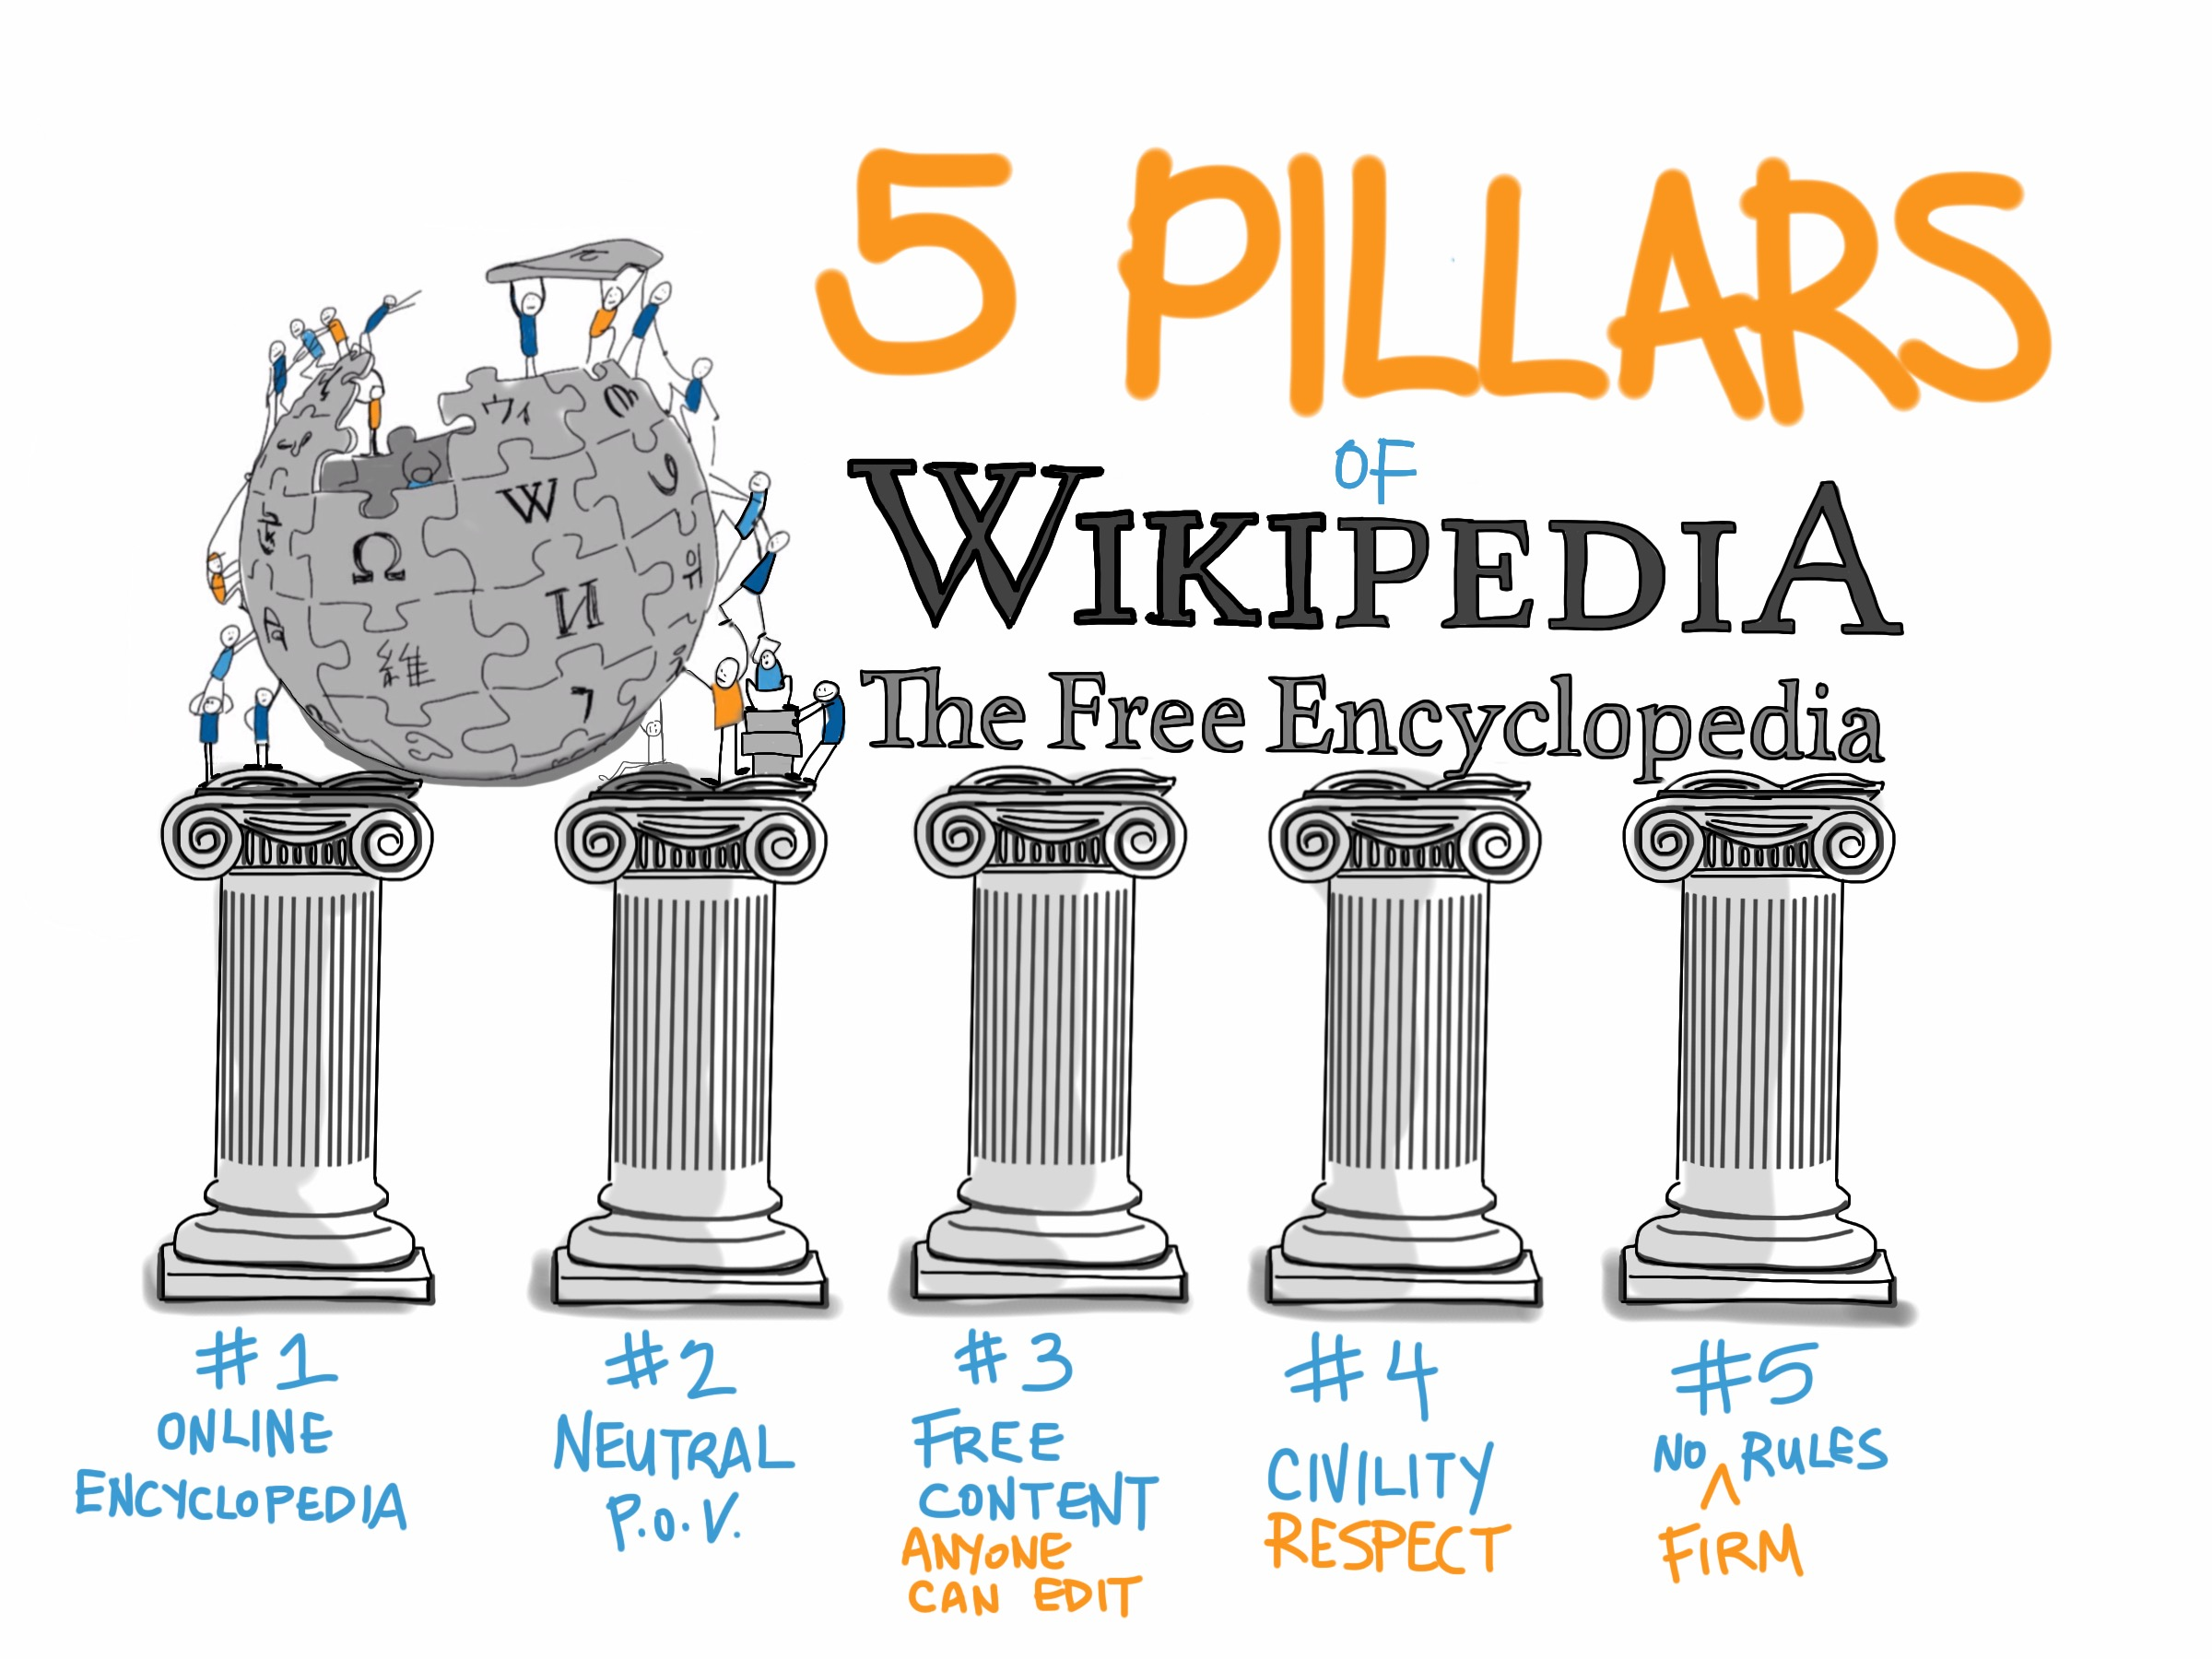
\includegraphics[width=0.75\textwidth]{images/Pillars.jpg}
    \caption{Five Pillars of Wikipedia. Image downloaded from \url{https://www.flickr.com/photos/gforsythe/21684596874}}
    \label{fig:5-pillars}   
\end{figure}

The first pillar states that Wikipedia is first and foremost an encyclopedia \cite{wiki:wiki-is-not}.
Therefore, it must not contain any original research, propaganda or advertisements \cite{wiki:wiki-NOR}.
Materials that do not have reliable references will be removed by other edits.

The second pillar specifies that articles on Wikipedia should strive for a neutral point of view.
This might include presenting multiple perspectives on the same subject accurately and not championing any one viewpoint as "correct" or "the truth".
If disagreements are present, then discussions must take place for building consensus.

The third principle enshrines the ideal that all content available on Wikipedia is free to edit and share.
However, this does not mean copyright violation and plagiarism is tolerated by the community.
There is no ownership of an article by an editor; anyone may freely modify any content.

The fourth pillar describes Wikipedia's code of conduct.
It asks users to act in good faith and assume good faith on the part of other editors.
Wikipedia etiquette urges disputes and disagreements, such as edit wars \cite{wiki:edit-wars}, to be resolved with civility while respecting other editors.

The fifth and last pillar reminds users that all rules in Wikipedia are essentially just policies and guidelines meant to help with collaboration.
They can evolve and change to reflect the requirement of the community.
It assuages the fear of making mistakes and encourages editors to be bold, though not reckless. 

\section{Formal Organization of Wikipedia}
\label{sec:formal-org-wikipedia}
In this section, we describe the various categories of users and explain their roles and responsibilities.
All the facts and figures we provide in this thesis are from the English version of Wikipedia.
We define a "user" of Wikipedia as a person who contributes to the encyclopedia and a "reader" as someone who simply accesses the content.

Wikipedia began as completely open platform with no restrictions on who could edit a page or create a new article.
Changes and edits that were made to a page were be published immediately.
This led to many pages that contained erroneous text, biased content and gibberish.
Therefore, this led to the English version of Wikipedia introducing restrictions and tools to protect the more controversial pages.
They also introduced categories of users to help protect and maintain the quality of the content available on Wikipedia.
We proceed to explain the four main user types as seen in Figure~\ref{fig:logos}. 
\begin{figure}[h!]
    \centering
    \begin{subfigure}[b]{0.49\textwidth}
        \centering
        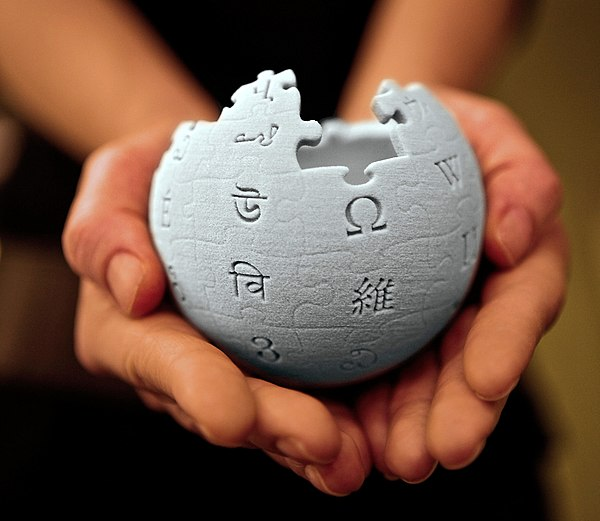
\includegraphics[width=0.5\textwidth]{images/wikipedians.jpg}
        \caption{Editors}
        \label{fig:editors}
    \end{subfigure}
    \begin{subfigure}[b]{0.49\textwidth}
        \centering
        
\includegraphics[width=0.5\textwidth]{images/admins.png}
        \caption{Administrators}
        \label{fig:admins}
    \end{subfigure}

    \begin{subfigure}[b]{0.49\textwidth}
        \centering
        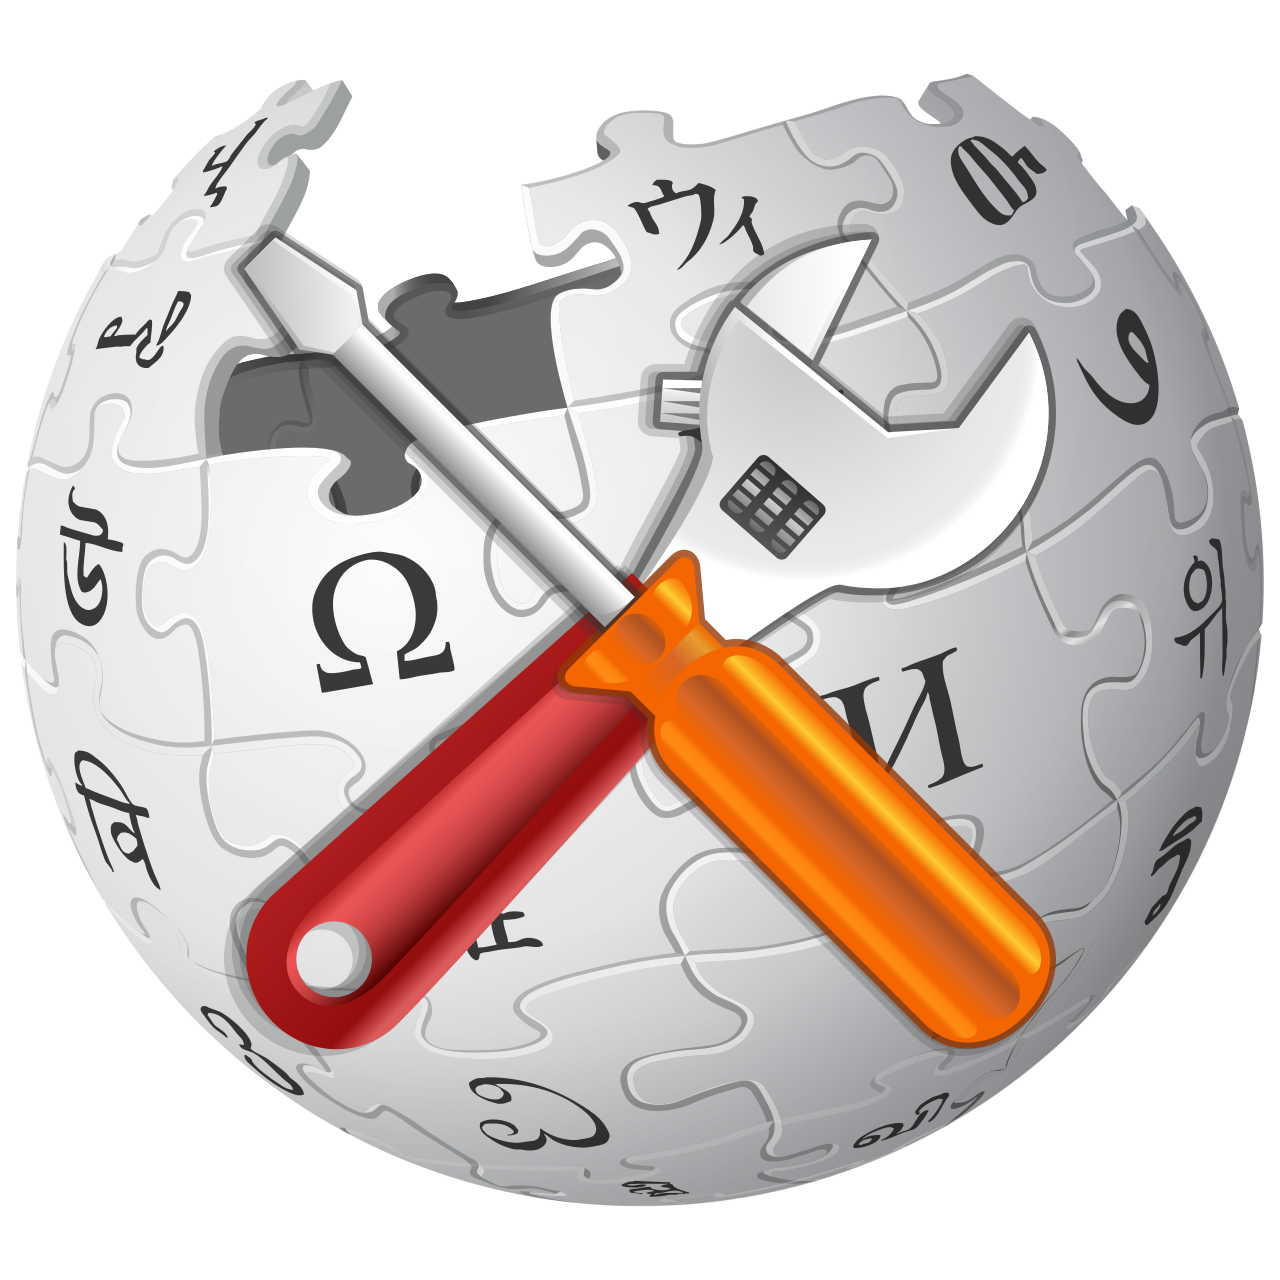
\includegraphics[width=0.5\textwidth]{images/bureaucrat.png}
        \caption{Bureaucrats}
        \label{fig:crats}
    \end{subfigure}
    \begin{subfigure}[b]{0.49\textwidth}
        \centering
        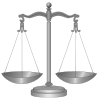
\includegraphics[width=0.5\textwidth]{images/arbcom.png}
        \caption{Arbitration Committee}
        \label{fig:arbs}
    \end{subfigure}
    \caption{Logos for each category of user that signify the role that they play in the Wikipedia community.}
    \label{fig:logos}
\end{figure}

\subsection{Editors}
\label{subsec:editors}
Editors (or Wikipedians) are the primary users who edit and create all the content on Wikipedia \cite{wiki:editors}.
Figuratively, they hold Wikipedia in the palm of their hands, as seen by the logo in Figure~\ref{fig:editors}.
There are two main types of editors on Wikipedia, namely \textit{registered} and \textit{unregistered}.
A registered user is someone who has a unique username and a permanent \textit{talk page} to communicate with other users.
By contrast, unregistered users contribute without a registered username and are usually referred to as \textit{IPs}, as they are only identified by their IP addresses.
Unregistered users usually have similar rights as those of regular users to edit, discuss and contribute, but with certain exceptions 
\cite{wiki:unregistered-users}.
Unregistered users cannot create a new article, edit a protected page, become administrators or vote in elections to promote users within Wikipedia.
As the focus of the thesis will be on the elections within Wikipedia, when we refer to editors in the coming chapters and sections, we refer to registered users.

Wikipedia has over 38 million registered users, and this number is constantly rising.
However, only roughly $0.37\%$ ($\approx 144\,000$) of registered users are active, i.e., have performed some action in the past 30 days.
An even smaller percentage of those active users participate in the community discussion forums on Wikipedia.
Now, we will explain what tasks editors perform and how contribution is recorded in Wikipedia.

Each page in Wikimedia is classified into a \textit{namespace} based on the type of information that page contains \cite{wiki:namespace}.
Namespaces separate pages into sets to distinguish content pages from administrative or editor related pages.
For example, the \mainNS (or \articleNS) namespace contains all the encyclopedic content and the \userNS namespace contains the user pages and information related to their user accounts.
Each page in Wikipedia also has a corresponding \textit{talk page}, which are used by editors to discuss changes to the page in question.
For instance, the \usertalkNS namespace has talk pages corresponding to each user page and acts as a system to message particular users.
Figure~\ref{fig:namespace} shows a list of the subject namespaces and their corresponding talk namespaces.
Now, we define a \textit{user contribution} as any addition, deletion or modification of a page under any namespace in Wikipedia \cite{wiki:user-contribs}.
Wikipedia collects and stores every user contribution so that it can track cases of vandalism and copyright infringement. 

\begin{figure}[htp]
    \centering
    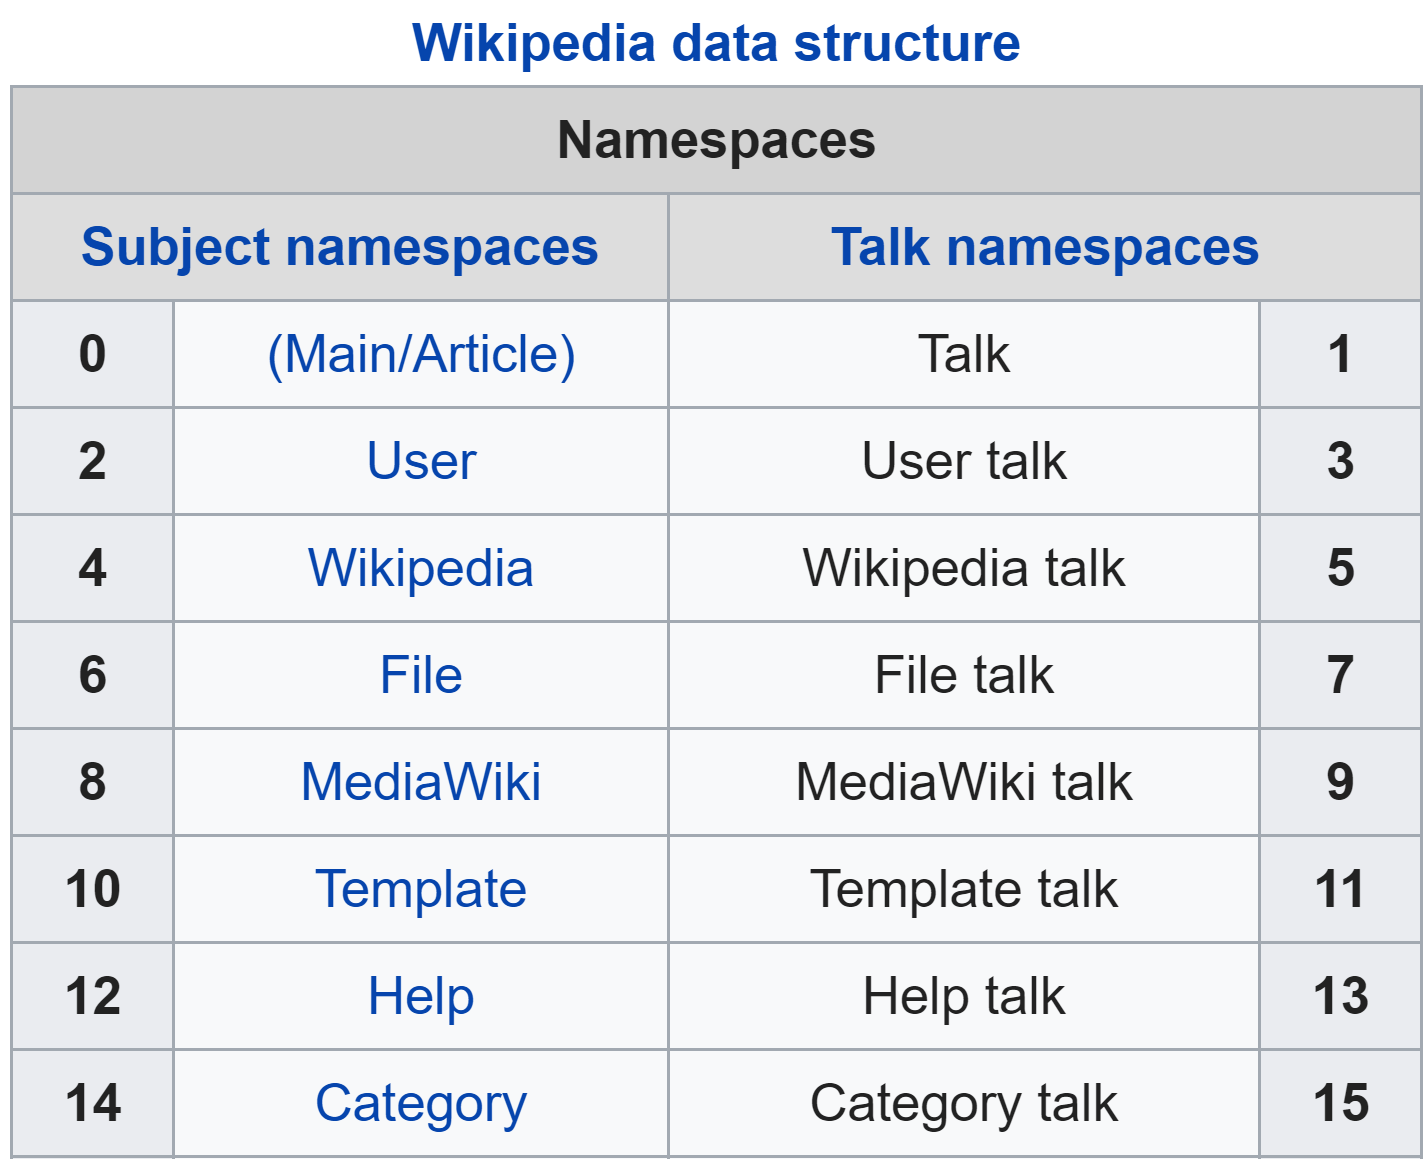
\includegraphics[width=0.75\textwidth]{images/namespaces.PNG}
    \caption{A list of the namespaces in Wikipedia \cite{wiki:namespace}.}
    \label{fig:namespace}
\end{figure}

The quality and quantity of the contribution of each editor varies significantly.
There are many occasional users who merely correct minor spelling and grammar errors in articles.
At the same time, there are dedicated editors who constantly create new articles, update large portions of text, and include new references and images.   

\subsection{Administrators}
\textit{Administrators} (or \textit{admins}) are editors who are given access to certain tools and powers to maintain content on Wikipedia.
Administrators can delete and restore deleted pages, block and unblock users and IP addresses from editing, and protect and remove protection from sensitive pages \cite{wiki:admins}.
These tools are associated with a mop that is used to clean up Wikipedia and is represented by their logo, seen in Figure~\ref{fig:admins}. 
There are currently 1\,141 administrators, of whom 500 are active.
Although admins have access to these tools, they are considered to be no more important than regular editors.
Administrators are elected through a week-long process called \textit{Request for Adminship} (RfA), at the end of which successful candidates are instated by a Bureaucrat.
We will cover the RfA process in detail in the coming sections. 

Along with the tools and power, administrators also have certain responsibilities.
They are not to misuse the tools at their disposal in conflicts of interest or disrupt Wikipedia by acting in bad faith.
Administrators serve indefinitely, but can be removed  by Bureaucrats on the decision of the Arbitration Committee for abuse of powers or inactivity.
Admins help with various areas of Wikipedia, such as processing administrative backlogs, helping with ant-vandalism efforts, and managing copyright issues. 

\subsection{Bureaucrats}
\textit{Bureaucrats} (or \textit{Crats}) are users who perform certain actions \cite{wiki:bureaucrats}.
They are usually administrators and oversee procedural rules and enforce decisions.
There are a total of 19 bureaucrats currently in the English Wikipedia.
Bureaucrats are involved in the granting or revoking of administrator status to users and adding and removing bots (software robots that carry out repetitive tasks on Wikipedia).
Bureaucrats are bound by the policy and the consensus of the community in granting these roles or permissions and are, therefore, expected to be good arbiters of consensus.
Hence, they should be able to identify criteria for a "consensus" and also explain the reasons behind their actions when requested. 

Bureaucrats are also elected through a process similar to RfA, called \textit{Request for Bureaucratship} (RfB), but higher thresholds of acceptance are usually demanded for considered selection.
Interestingly, Bureaucrats are also appointed following the final decision of another Bureaucrat, therefore, they have complete control over the whole process.
However, a Bureaucrat cannot revoke the bureaucratic position of others.
They also carry out the requests from the Arbitration Committee to remove the permissions and privileges of admins or bots.
As their name suggests, Crats perform only bureaucratic duties and are therefore represented by the logo seen in Figure~\ref{fig:crats}.

\subsection{Arbitration Committee}
The \textit{Arbitration Committee} (or \textit{ArbCom}) resolves disputes that have not reached a resolution through community discussion or administrator oversight \cite{wiki:arbcom}.
Their goal is to decisively bring binding solutions to ongoing disputes and is reflected in the fact their logo is a balance scale, as seen in Figure~\ref{fig:arbs}.
It is formed by a panel of experienced editors, usually administrators, who are elected by the community annually.
There are currently 11 active members of the ArbCom.

The ArbCom only deals with disputes related to editor conduct and not content related disputes.
It can impose sanctions that would restrict editors from contributing to certain topics and also recommend the revoking of administrative privileges in cases of misuse.
Although the ArbCom can take the initiative on matters it deems are important, it usually acts on formal requests made to the committee.
As it is the last step in dispute resolution, it only accepts a case when all other methods have failed.
This is evident from the fact that only 9 cases were accepted in 2019. 

\section{Request for Adminship}
\label{sec:rfa}
In this section, we will describe the election process to select administrators in the English version of Wikipedia called \textit{Request for Adminship} (RfA).
We cover the origin and history of the process, the evolution of the format and the properties that lead to successful candidates.
Lastly, we also cover the existing research that has been carried out in understanding and predicting RfAs.

In the early days of Wikipedia, the founder, Jimmy Wales, directly sent emails to the users to appoint them as administrators.
Jimmy said that he felt that getting administrative privileges is "not a big deal".
However, as the Wikipedia community grew, a long and intense process was developed to select future administrators.
A RfA is a week-long period during which all registered Wikipedia users can vote on a candidate standing for the position of administrator. 

There are four main phases of a RfA: the nomination and beginning the period, answering questions posed by the community, voting to show support, opposition or neutrality towards the candidate, and the closing of the RfA by a Bureaucrat.

The first phase begins with the creation of a RfA page for the nominee.
The candidates are most often nominated by another well-known and respected editor.
However, self-nomination is a possibility.
Self-nominated candidates are usually under more scrutiny to ensure they are not overeager new users nor editors with prior issues.
Nominations are usually accompanied by an introductory statement from the nominator indicating the qualities the candidate possesses.
Nominees can decline a nomination if they wish to, in which case the RfA is closed immediately as unsuccessful.
Therefore, nominators usually only choose candidates who show good promise and discuss the potential nomination prior to starting the RfA process. 

Once a candidate accepts the RfA nomination, they are required to answer three standard questions. 
\begin{enumerate}
    \item What admin work do you intend to take part in?
    \item What are your best contributions to Wikipedia, and why?
    \item Have you been in any conflicts over editing in the past or have other users caused you stress? How have you dealt with it and how will you deal with it in the future?
\end{enumerate}
The first question aims to discern the value addition that a particular candidate will bring to Wikipedia if given admin privileges.
The community tends to look for initiative from nominees in utilizing existing tools to help with chores such as reverting errors, identifying vandalism or copyright infringements.
The answer to the second question provides the community the candidate's achievements and quality of work.
Editors who have several multiple good contributions tend to be more successful.
In answering the third question candidates demonstrate their conflict management skills.
The community values users who can interact in a civil manner and an administrator is also involved in resolving disputes and therefore, users who were involved in heated discussions or edit wars are unfavourable.
Apart from these three fixed questions the candidate may also receive several open questions aimed at testing their knowledge of Wikipedia procedures or opinions on controversial issues.

Once all questions have been answered, the RfA moves to the voting phase.
During this phase, any registered user may vote in either Support, Oppose or Neutral sections.
Votes are generally followed by a comment providing reasoning that explains their vote.
Candidates can reply to opposition commenters to try and resolve any issues and convert their views.
However, candidates should refrain from verbose rebuttals as it might invite more opposition.
This phase is nerve-racking for the candidate as the tide of the election changes constantly throughout the week and it is not possible to reply to every comment in a civil and respectful manner.

At any point in the RfA, the candidate can withdraw their nomination for any reason.
At the end of the week, a Bureaucrat halts the voting and proceeds to read all the comments.
The Bureaucrat has to conclude if consensus has been reached or not regarding the nomination.
Bureaucrats are highly experienced and will discount votes cast by sockpuppets (users who have multiple accounts) and meatpuppets (new users recruited to influence decisions).
Although the decision is not based on majority voting, RfAs with more than $75\%$ support generally pass and by contrast ones with lesser than $65\%$ support are bound to fail.  

The Bureaucrat can also invoke clauses such as "Not Now" (WP:NOTNOW \cite{wiki:wp:notnow}) and "Not a snowball's chance in hell" (WP:SNOW \cite{wiki:wp:snow}) to terminate RfAs that they deem have no chance to pass.
These measure exists so that frivolous RfA do not waste the time of the community.
If the Bureaucrat decides that the nomination is successful, the candidate is promoted and the RfA is closed as successful.
If the nomination fails then the Bureaucrat explains their reasoning and closes the RfA as a failure.
Renomination of a failed candidate can occur after waiting for a reasonable period of time from the previous failed RfA.

RfAs have been extensively studied from a sociological and behavioural aspects \cite{derthick2011collaborative,kordzadeh2016revisiting}.
Burke et al.\ \cite{burke2008mopping} proposed a model based on RfA guides to predict the success of a potential nomination.
Since then, there have been various models based on social networks  \cite{putzke2017stated,cabunducan2011voting,picot-clemente2015social} or user features and contributions \cite{clemente2015contribution,asim2018personal} to identify influential voters and overall voting patterns. 


\chapter{Results and Discussion} 
\label{chp:results}
In this section we will present the results of the models and discuss their implications.
\section{Linear Combination of Graphs}
\begin{itemize}
    \item Present results for each linear classifier
    \item Discuss the different splits of the dataset to check for robustness and chronological consistency
    \item Show the feature importances and discuss their relevance 
    \item Compare the raw accuracy versus the macro f1 scores
    \item Highlight the difficulty of predicting negative votes
\end{itemize}
\section{Local Signed Network}
\begin{itemize}
    \item Present the Iterative Balance model results
    \item Discuss quality of predictions using evaluation metrics
    \item Mention the difference between deterministic and probabilistic prediction accuracies
    \item Explain the Iterative Status model results 
    \item Discuss the issues with local model of status and the potential reasons for lower score and quality
\end{itemize}
\section{Voting Order Results}
\begin{table}
    \centering
    \caption{Results for different vote orderings for the failed RfA}
    \label{tab:fail-rfa}
    \begin{tabular}{llccc}
        \toprule
        Model & Vote Order & ROC AUC & PR Positive  & Pr Negative \\ \midrule
        Baseline & - & 0.5 & 0.52 & 0.479 \\
        \midrule
        
        \multirow{3}{*}{\shortstack[l]{Iterative\\ Balance}} & 
        Normal &  0.543 & 0.74 & 0.454 \\
        \cmidrule{2-5}
        &Reversed & 0.74 & 0.868 & 0.572 \\
        \cmidrule{2-5}
        & Random & 0.68 & 0.812 & 0.575 \\
        \midrule

        \multirow{3}{*}{\shortstack[l]{Iterative\\ Status}} & 
        Normal & 0.962 & 0.977 & 0.909 \\
        \cmidrule{2-5}
        & Reversed & 0.930 & 0.965 & 0.806   \\
        \cmidrule{2-5}
        & Random & 0.924 & 0.957 & 0.818 \\
        \bottomrule
        \end{tabular}
\end{table}

\begin{table}
    \centering
    \caption{Results for different vote orderings for the successful RfA}
    \label{tab:pass-rfa}
    \begin{tabular}{llccc}
        \toprule
        Model & Vote Order & ROC AUC & PR Positive  & Pr Negative \\ \midrule
        Baseline & - & 0.5 & 0.905 & 0.095 \\
        \midrule
        
        \multirow{3}{*}{\shortstack[l]{Iterative\\ Balance}} & 
        Normal &  0.9175 & 0.991 & 0.385 \\
        \cmidrule{2-5}
        &Reversed & 0.720 & 0.972 & 0.142 \\
        \cmidrule{2-5}
        & Random & 0.894 & 0.989 & 0.431 \\
        \midrule
        
        \multirow{3}{*}{\shortstack[l]{Iterative\\ Status}} & 
        Normal & 0.846 & 0.981 & 0.293 \\
        \cmidrule{2-5}
        & Reversed & 0.895 & 0.99 & 0.29 \\
        \cmidrule{2-5}
        & Random & 0.931 & 0.992 & 0.451 \\
        \bottomrule
        \end{tabular}
\end{table}
\section{Comparison}
\begin{itemize}
    \item Compare results from signed edge prediction and Iterative signed models
    \item Discuss Static Linear combination predictions versus Iterative signed predictions 
    \item Discuss the assumptions used in the models and limitations 
\end{itemize}

\chapter{Conclusions and Future Work}
\label{chp:conclusion}
\begin{itemize}
    \item Explain the quality of results with the election perspective
    \item Future work is to extend this to other election settings and investigate generality of this approach
    \item Possible future work in congressional voting data
    \item Can also tackle the other problem in information cascade theory of how to predict who is most likely to vote next 
    \item This can lead to a complete model of election dynamics and could incorporate elements of game theory and network inference 
\end{itemize}

 
% \chapter{Implementation}
\label{chp:implementation}
In this chapter, we will outline the experiments carried out on the Wikipedia elections of administrators using the vote prediction models that we presented in chapter~\ref{chp:vote-prediction}.
Firstly, we describe the existing sources of data from Wikipedia and the datasets used in the experiments in Section~\ref{sec:datasets}.
Next, in Section~\ref{sec:linear-combination-implementation}, we discuss the implementation of the linear combination of graphs model described in Section~\ref{sec:linear-combination-theory}.
Then, we cover the implementation of the vote prediction models based on the theories of balance and status in signed networks in Section~\ref{sec:local-signed-network-implementation}.
Furthermore, in Section~\ref{sec:voting-order}, we discuss the experiments conducted on the voting order and its impact on the predictive power of the models proposed.
Lastly, we explain the metrics which we can use to evaluate the performance of the models in Section~\ref{sec:eval-metrics}.

All implementations and datasets can be found at \url{https://github.com/ananth1996/Wikipedia}
\section{Datasets}
\label{sec:datasets}
As we discussed in Section~\ref{sec:rfa} and \ref{subsec:editors}, Wikipedia keeps detailed information on the election proceedings for the RfA process as well as contributions made by every editor on Wikipedia.
These act as sources to get data regarding the elections and user contributions. There are existing datasets compiled by the Stanford Network Analysis Project (SNAP) \cite{snapnets} on both Wikipedia RfAs and edit histories.
However, the RfA dataset has missing features and timestamps for votes that would restrict the usability in the proposed voting models.
Similarly, the \textit{wiki-meta} and \textit{wiki-talk} datasets only possess information until 2008 and lack a username mapping to the network nodes.
Due to these limitations, we proceeded to scrape Wikipedia dumps and APIs to obtain our own RfA and user contribution datasets, which we will now describe.

\subsection{Wikipedia RfA Data}
To obtain the RfA data, we parsed through the entire XML dump of Wikipedia from January 2019.
We filtered the pages related to the RfA process and then extracted each vote and the corresponding comment and timestamp.
Each vote extracted has the features shown in Table~\ref{tab:wiki-rfa-features}.

\begin{table}[htp]
    \centering
    \caption{Features of each vote in the \wikirfa dataset}
    \label{tab:wiki-rfa-features}
    \begin{tabular}{ccc}
        \toprule
        Feature & Data Type & Description\\
        \midrule
        \textbf{SRC}&text & username of the source\\
        \textbf{TGT}&text & username of the target\\
        \textbf{VOT}&$[-1,0,1]$& Oppose, Neutral or Support vote\\
        \textbf{RES}&$[-1,1]$ & Failure or Success of RfA\\
        \textbf{YEA}&date & year of the RfA\\
        \textbf{DAT}& date \& time & timestamp of the vote\\
        \textbf{TXT}&text &accompanying textual comment \\
        \textbf{UID}&alphanumeric&  unique identifier for the RfA\\
        \bottomrule
    \end{tabular}
\end{table}
As we can see, the format of the data is very similar to the SNAP dataset.
We have an additional unique identifier field, called UID, to aid in distinguishing RfA of users who have had multiple nominations.
We collected $226781$ votes from $4557$ elections with over $13000$ unique usernames. There are $166214$ ($\approx 73\%$) support, $46918$ ($\approx 20\%$) oppose and $13649$ ($\approx 6\%$) neutral votes.
As the voting format of RfA changes throughout the years, there were issues in successfully extracting the source username or timestamp information. 
Regardless, only $1.6\%$ of votes have missing timestamps and $0.4\%$ have a missing source.
We will refer to this dataset as \wikirfa and it will provide the information regarding the votes cast in a RfA.

\subsection{User Contribution Data}
As we discussed in Section~\ref{subsec:editors}, every edit made by a user is stored as a contribution.
Wikipedia provides an API to query all the contributions of a particular user \cite{wiki:Usercontribs-api}.  
We utilized this API and collected the contribution data of all the unique users we obtained from the \wikirfa dataset.
There are 16 features that the API provides for each edit; we describe the most import features in Table~\ref{tab:usercontrib-features}.

\begin{table}[htp]
    \centering
    \caption{Important features of each contribution in the \usercontrib dataset}
    \label{tab:usercontrib-features}
    \begin{tabular}{lcc}
        \toprule
        Feature & Data Type & Description\\
        \midrule
        \textbf{user}&text& username of the editor\\
        \textbf{title}&text & title of the page edited\\
        \textbf{namespace}&int& namespace of the page edited\\
        \textbf{timestamp}&date \& time & timestamp of the edit\\
        \textbf{size}&int& new size of the edit \\
        \textbf{sizediff}& int & size delta of the edit against its parent\\
        \textbf{new}&boolean &if the editor created a new page \\
        \textbf{minor}&boolean& if it is a minor edit\\
        \textbf{comment}& text& accompanying comment\\
        \bottomrule
    \end{tabular}
\end{table}
As many users change their username, some of the usernames present in the \wikirfa dataset might not have any contributions linked to their old usernames.
We were able to collect the user contribution details of more than $11000$ users, amounting to 100GB of data.
We call this dataset \usercontrib and it provides a wealth of information on the editing habits of the users who take part in Wikipedia RfAs. 
For instance, grouping the contributions of a particular user by the namespace, we get the proportion of the edits in different Wikipedia namespaces and the respective sizes and quality of their edits.

\section{Graph Combination Model}
\label{sec:linear-combination-implementation}
In this section, we describe how we implemented the linear combination of graphs framework proposed in Section~\ref{sec:linear-combination-theory} for predicting votes in Wikipedia RfA elections.
We call this the \textit{Graph Combination} model.
The model requires auxiliary graphs created from other non-election based information as well as triadic features extracted from the voting data.
Firstly, we discuss the auxiliary graphs that we create from the \usercontrib dataset.
Next, we explain the nomenclature and collection of triadic features from the \wikirfa data.
Then, we describe the process of preparing the data to suit the supervised machine learning task as well as preventing any potential data leaks.
Lastly, we discuss the logistic regression model that we use as the linear classifier trained on the features derived from the auxiliary and signed networks.

The terms used in Chapter~\ref{chp:vote-prediction} can now be defined for the problem of predicting votes in a Wikipedia RfA.
A candidate $c$ is the nominee who wishes to gain administrators privileges in the Wikipedia RfA.
The voters $v$ are the registered users in Wikipedia.
A session relates to the proceedings of a particular RfA.
\subsection{Graphs}
First, we discuss the creation of the topic similarity network of users.
Then, we describe the process of forming the talk graph between users.
Lastly, we define the triadic features we extract from the previous voting data. 

\subsubsection{Topic Similarly Graph}
In Table~\ref{tab:usercontrib-features}, we see that every contribution has a title of the page where the edit was made.
The most edited page titles of a user help in understanding the topics they are interested in.
Therefore, for a particular user, we gather all their edits in the \mainNS namespace.
We choose the \mainNS namespace as it contains all the content articles on Wikipedia.
By contrast, a user's edits in other namespaces such as, \userNS and \helpNS, are not indicative of the topics in which they possess knowledge.
Then, we count the number of edits grouped by each page title and choose their top 100 most edited pages in the \mainNS namespace.
Then we create a set of the words from all the top 100 page titles and remove common stop words using a natural language corpus.
This set now indicates the user's topics of interest.
Once we have collected the topic set for all the unique users in the \wikirfa dataset, we can compute the similarity between a pair of users using the Jaccard similarity measure. 
Then, we can take this similarity measure and construct a undirected weighted graph where a link between any two nodes indicates the similarity in the topics of the corresponding users.
However, we threshold the value of similarity so that we can obtain only meaningful edges and not a complete graph.

\subsubsection{Talk and Interaction Graph}
\label{subsec:talk-interaction-graph}
We discussed in the previous chapter how every registered user has a talk page and how it is used as a medium of communication. 
Therefore, we can gather the contributions of a certain editor in the \usertalkNS namespace and use it to measure their interactions with other users.
We will create two auxiliary graphs in this manner.
The first is a \textit{user talk graph}, where each edge contains the number of times they have written on another user's page.
The second is a \textit{interaction graph}, in which an edge only indicates if two users have interacted via a talk page. 
We can obtain the number of talk page edits and the target user by grouping by the page titles and extracting the username from the page title respectively. 
These graphs will be directed in nature and the talk graph is weighted, while the interaction graph is unweighted. 
In both these graphs, an edge $u \rightarrow v$ indicates that user $u$ has written in the talk page of user $v$.

In the Line~\ref{alg:aux:voting-neighbourhood} of Algorithm~\ref{alg:auxiliary-feature}, we compute the neighbourhood of a node $v$ in graph $G_i$ as $N_i$.
We can define $N_i$ in directed graphs $G_i$ as only the successors of a node rather the union of successors and predecessors.
This allow us to understand the influence of edge direction in directed auxiliary graphs.
Therefore, we will construct two more additional auxiliary graphs which are \textit{reversed}, i.e., an edge $u \rightarrow v$ indicates that user $v$ has written on the talk page of user $u$.
Hence, we can compare the benefit each direction brings to the model by analysing the feature importances of their respective auxiliary graphs.

\subsubsection{Signed Graph and Triadic Features}
The \wikirfa dataset contains the voting information of users in RfAs.
These votes form a signed directed network.
Therefore, we can utilize the triadic features framework as proposed by Leskovec et al.\ \cite{leskovec2010predicting}.

We utilize a slightly modified naming scheme to identify unique triads in the RfA data.
Consider the we have a voter $v$, a candidate $c$ and a third node $u$.
Then, the edge we wish to predict is $(v,c)$ and the other edges $(v,u)$ and $(u,c)$ form a triad.
There are two directions for the edges $(v,u)$ and $(u,c)$ and each edge can have three values, namely -1, 0 or +1 corresponding to a oppose, neutral or support vote respectively.
This leads to $2 \times 2 \times 3 \times 3 = 36$ possible triads.

We denote the edge $v \rightarrow u$ as "F" and the edge $v \leftarrow u$ as "B" indicating a forward or a backward edge respectively.
Similarly, the edge $u \rightarrow c$ is "F" and $u \leftarrow c$ is "B".
The edge labels are "-", "0", or "+" corresponding to a oppose, neutral or support vote.
Therefore, using this nomenclature, the triad "FB+-" represents the edges $v\plusrightarrow c$ and $u \minusleftarrow c$.
Figure~\ref{fig:triad-naming} shows more examples of this triad nomenclature.

\begin{figure}[htp]
    \centering
    \tikzset{
    position/.style args={#1:#2 from #3}{
        at=(#3.#1), anchor=#1+180, shift=(#1:#2)
    }
}

\begin{tikzpicture}

    \begin{scope}[every node/.style={circle,thick,draw}]
        \node (v2) at (0,0) {$u$};
        \node[position=-120:1cm from v2] (v1) {$v$};
        \node[position=-60:1cm from v2] (v3) {$c$};
        
        \node[right=2.5cm of v2] (v5) {$u$};
        \node[position=-120:1cm from v5] (v4) {$v$};
        \node[position=-60:1cm from v5] (v6) {$c$};
        
        \node[right=2.5cm of v5] (v8) {$u$};
        \node[position=-120:1cm from v8] (v7) {$v$};
        \node[position=-60:1cm from v8] (v9) {$c$};
    
        

    \end{scope}

    \begin{scope}[>={Stealth[black]},
        positive/.style={thick,draw,->},
        negative/.style={thick,draw,->},
        pred/.style={thick,dashed,draw,->,dashed},
        every node/.style={fill=white,circle}]
        % \draw (v4) -- (v1) -- (v3) -- (v2) -- (v1);
        \path 
        (v1) edge[positive] node[above left=0.1mm and 0.1mm] {$+$} (v2)
        (v2) edge[positive] node[above right=0.1mm and 0.1mm] {$-$} (v3) 
        (v1) edge[pred](v3)   

        (v5) edge[negative] node[above left=0.1mm and 0.1mm] {$-$} (v4)
        (v5) edge[negative] node[above right=0.1mm and 0.1mm] {$0$} (v6) 
        (v4) edge[pred] (v6)      
        
        (v7) edge[positive] node[above left=0.1mm and 0.1mm] {$0$} (v8)
        (v9) edge[positive] node[above right=0.1mm and 0.1mm] {$+$} (v8) 
        (v7) edge[pred] (v9)      
        ;
        
    \end{scope}

    \begin{scope}[
        every node/.style={fill=white,rectangle},
        every edge/.style={fill=white}
        ]
        \path 
            (v1) edge node[below=1cm] {$FF+-$}  (v3) 
            (v4) edge node[below=1cm] {$BF-0$} (v6)      
            (v7) edge node[below=1cm] {$FB0+$} (v9)      
            ;     
    \end{scope}
  \end{tikzpicture}
  
    \caption{Examples of triad nomenclature in Wikipedia RfA elections. Dashed edges are votes to be predicted and solid edges are votes from previous RfAs.  }
    \label{fig:triad-naming}
\end{figure}
We store all the 36 unique triads in the set $T$ and then utilize it to count the triads for a particular edge, as seen in Algorithm~\ref{alg:triad-feature}.
Therefore, for each edge to be predicted $(v,c)$, we have a triadic feature vector of length 36 containing the counts of the triads formed by all the common neighbours $u$.  

\subsection{Data Preparation}
\label{subsec:data-prep}
As only roughly $6\%$ of all votes are neutral votes, we will not try to predict neutral votes.
This is in line with the Wikipedia RfA process where neutral votes are not counted for the support percentage. 
However, we will use the neutral votes to gather the triadic features and can utilize the additional information to predict votes.

As we discussed in Section~\ref{sec:voting-signed-networks}, the graph combination model is an extension of a sign prediction model for the task of predicting votes.
A major requirement to predict votes is to ensure that there is no \textit{data leakage} when creating the training features $\mathbf{X}$.
A data leak is when we have information about the future available in the training data.
This can cause the model that we train to overfit on the leaked data and not generalize.
Kairimi et al.\ \cite{karimi2019multicongress} outline a process to split a dataset chronologically and gather information respecting the boundary dates at the location of the splits.
Similarly, for our problem setting, we divide the whole \wikirfa into three parts, namely \textit{dev}, \textit{train} and \textit{test}.
As we are predicting votes, we split the datasets based on the number of votes chronologically and round up to the closest RfA so that it is contiguous. 

The \textit{dev} (or development) dataset will be the set of RfAs which we use to construct the auxiliary and signed graphs.
We ensure that the \usercontrib dataset is also restricted to the edits that happened until the date of the last RfA in the dev dataset.
Therefore, all the five auxiliary graphs and the signed graphs are created only with information that is present in the time frame of the dev dataset.

Next, the \textit{train} (or training) dataset is what we use to create the feature matrix $\mathbf{X}$ and target matrix $\mathbf{y}$.
In this dataset, we only consider the support and oppose votes to be part of the prediction task and hence, filter out all the neutral votes.
Now, for each vote, we create the auxiliary feature vector $\textbf{a}$ using the five auxiliary graphs and the triadic feature vector $\mathbf{t}$ from the signed voting graph as described in Algorithms~\ref{alg:auxiliary-feature} and \ref{alg:triad-feature} respectively.
These features are concatenated into a feature vector $\textbf{x}$, which is of length $41$ ($5$ auxiliary and $36$ triadic features) and is a row of the feature matrix.
The corresponding true vote is also collected in the target $y$.
The \textit{dev} split ensure that the auxiliary and triadic features in \textit{train} do not overlap with the \textit{test} split.
Therefore, this allows the feature matrix $\textbf{X}$ to be independent of time and we can use methods such as $k$-fold to cross validate the model.

Lastly, the \textit{test} dataset contains votes that the model trained on the training dataset would not have seen.
This can be used to evaluate the performance of the model.
The feature matrix for the test dataset, $\mathbf{X}_{test}$ and the target, $\mathbf{y}_{test}$ are also constructed in a similar manner.
For each vote in the test dataset, we gather the auxiliary and triadic features from the same graphs as we used for the training phase.
We create each row of $\mathbf{X}_{test}$ by concatenating these features and gathering the true votes as the target.

As the auxiliary features and triadic features have different ranges, we standardize both training and testing feature matrices so that all features have a mean of zero and standard deviation of one.
This will help the linear models train better and reach an optimal solution faster as well as allow for ease in interpreting the coefficients of the linear model.

\subsection{Supervised Classification}
Once we have created the training and testing feature matrices, $\mathbf{X}$ and $\mathbf{X}_{test}$ and the target vectors, $\mathbf{y}$ and $\mathbf{y}_{test}$, the task is a regular supervised classification problem.
We can use any traditional linear classification model such as support vector classifier (e.g.,linear SVC), logistic regression model or gradient boosting method (e.g., XGBoost).
We choose a logistic regression (LR) model for its interpretability and robustness to overfitting. 

Given a feature vector $\mathbf{x}=(x_{1},x_{2},\dots,x_{n})$ with $n$ features, a logistic regression model learn to predict the probability of the form 
\begin{equation}
    P(\text{support} \mid \mathbf{x}) = \frac{1}{1+e^{-(\beta_{0} + \boldsymbol{\beta}\mathbf{x}})}
\end{equation}
Where $\beta_{0}$ and $\boldsymbol{\beta} = (\beta_{1},\beta_{2},\dots,\beta_{n})$ are the coefficients that the model learns using the training data.

The \wikirfa dataset has a class imbalance problem.
Support votes are $73\%$ compared to oppose votes at $20\%$.
Therefore, we will utilize class weights inversely proportional to the class frequencies while training so that the model learns to predict negative votes effectively. 
As the training features $\mathbf{X}$ are independent of time, we use $k$-fold cross validation to tune the regularization parameter for the logistic regression model.  

\section{Local Signed Network Models}
\label{sec:local-signed-network-implementation}
We now discuss the implementation of the local signed network models discussed in Section~\ref{sec:local-signed-network-theory} to predict votes in Wikipedia RfAs.

These models are iterative models and an important feature is that they are unsupervised.
Therefore, they do not require any learning of parameters or preparation of data for training.
Consequently, we can bootstrap the models to start from the first available RfA.
We achieve this by beginning with an empty relationship graph $R$.
In the first RfA, the LSN for all the votes contain only the nodes for voter $v$ and candidate $c$.
Therefore, the model will predict all votes with probability $0.5$ of being support votes, as there is no information available.
After the first RfA is over, the relationship graph $R$ will be updated with the voting details.
Now, in the second RfA there is more information present and the model can predict votes with more certainty.
In this manner, the models can iteratively learn and predict all the votes present in the \wikirfa dataset.

In a similar fashion, the iterative models elegantly handles new users for whom we have no information .
If at any point the current voter $v$ is new and there is no information in the relationship graph , then the model predicts support vote probability of $0.5$, because the LSN contains only the nodes $v$ and $c$ .
This new voter is then integrated into the relationship graph when it is updated after the RfA session, shown in Line~\ref{iterative-pred:line:update-relation} of Algorithm~\ref{alg:iterative-pred}.
Therefore, this new voter's information is now available for future vote predictions.

In this thesis, we wish to separately study the votes that are predicted with no information.
Therefore, in our implementation we specifically mark these votes.
Consequently, we can accurately evaluate the iterative model using only the votes predicted with information.
Then, we can analyse the distribution of the informationless votes and devise strategies to effectively guess the vote in the cases when a voter is new.
Lastly, we can verify if there new voters follow some herd mentality when they vote for the first time.

We proposed two iterative models in Section~\ref{sec:local-signed-network-theory}, one using balance theory and another using status theory.
Both these models make use of only the votes cast in sessions.
Therefore, we will use the \wikirfa dataset for the iterative models.
First, we describe the iterative balance model and define the relationship graph based on \textit{agreement} between voters in Wikipedia RfAs.
Secondly, we explain the iterative status model and the relationship graph based on the \textit{follower ratio} in RfAs.

\subsection{Iterative Balance Model}
The \textit{Iterative Balance Model}  uses balance theory in the local signed network to predict the votes of independent voters in a Wikipedia RfA.
As discussed in Section~\ref{subsec:prediction-based-balance}, we require a signed symmetric measure between two voters.
We now propose a measure based on the \textit{agreement ratio} between two users $u$ and $v$.
The ratio is the number of times $u$ and $v$ have voted similarly, divided by the number of common RfAs they have participated in.
For example, if $u$ and $v$ have participated in $12$ common RfAs and have voted the same in $9$ RfAs, then the agreement ratio is $0.75$.
This indicates that they agree more than they disagree.
Therefore, if a pair of users have an agreement ratio of $0.5$, then they neither agree or disagree with each other.
The agreement ratio is symmetric and we covert it into a signed measure by subtracting 0.5 from the ratio.

Hence, we define a signed undirected \textit{agreement graph} $A= (V_{A},E_{A},w_{A})$, where the weight function is defined as seen in Equation~\eqref{eqn:agree-weight}.
\begin{equation}
    \label{eqn:agree-weight}
    w_{A}((u,v)) = \frac{\text{Number of times } u \text{ and } v \text{ have voted similarly}}{\text{Number of common RfAs for } u \text{ and } v} -0.5
\end{equation}

This agreement graph $A$, is the relationship graph $R$ for the iterative balance model described in Algorithm~\ref{alg:iterative-pred}. 
In Line~\ref{iterative-pred:line:update-relation} there is a a method, $Update(R,S)$ to update the relationship graph after the end of a voting session.
Therefore, we require a method to update the signed weights in the agreement graph $A$ given the RfA voting details in a session $S$.

For notational ease, we assume that each edge $e = (u,v) \in E_{A}$ contains two attributes, $e.agree$ and $e.common$, the agreement ratio and the number of common RfAs between the nodes respectively.
Then, once we get the voting information from the session, we can update the agreement ratio and the number of common RfAs in a straightforward manner.
This process is shown in Algorithm~\ref{alg:agree-update}.

We can bootstrap the model by beginning with an empty agreement graph $A$.
Then for votes with no information the predicted support probability is $0.5$.
After the RfA session is over, these new voters will be incorporated into the agreement graph.
Therefore, from the next RfA, the model has information on the voters it has now incorporated.

\begin{algorithm}[htp]
    \DontPrintSemicolon
    \caption{Update Agreement graph after a session}
    \label{alg:agree-update}
    \KwIn{Session graph $S$, Candidate $c$, Agreement graph $A$ }
    \KwResult{Updated Agreement graph $A$ }
    \tcp{Get all voters}
    $O \leftarrow V_{S}-\{c\}$\;
    Order $O$ by timestamp\;
    \For{$v \in O$}{
        $vote_{v}\leftarrow w_{S}((v,c))$\;
        \ForEach{$u$ who voted after $v$}{
            $vote_{u} \leftarrow w_{S}((u,c))$\;
            $e \leftarrow (v,u)$\;
            \uIf{$e \in E_{A}$}{
                $agree \leftarrow e.agree$\;
                $common \leftarrow e.common$\;
                \eIf{$vote_{v}=vote_{u}$}{
                    $agree \leftarrow ((agree\cdot common) +1)/(common+1)$\;
                }{
                    $agree \leftarrow (agree\cdot common)/(common+1)$\;
                }
                $common \leftarrow common +1$\;
            }
            \ElseIf{$vote_{u}=vote_{v}$}{
            \tcp{if $e$ is a new edge}
            \label{alg:agree-update:new-edge}
            $common \leftarrow $ number of elections $v$ and $u$ have in common\;
            $agree \leftarrow 1/common$\;
            $E_{A} \leftarrow E_{A} \cup \{e\}$
            }
            $e.agree \leftarrow agree$\;
            $e.common \leftarrow common$\;  
            $w_{A}(e) \leftarrow e.agree -0.5$\;
        }
    }
    \Return $A$
\end{algorithm}

\subsection{Iterative Status Model}
The \textit{Iterative Status Model}, as described in Section~\ref{subsec:prediction-based-status}, utilizes status theory in the LSN to predict votes.
Therefore, to predict votes in Wikipedia RfAs, we require a directed signed relationship graph.
Similar to the agreement ratio for the iterative balance model, we propose a \textit{follower ratio} and a corresponding directed singed \textit{follow graph} $F=(V_{F},E_{F},w_{F})$.

An edge $u \rightarrow v$ in $F$ indicates that node $u$ follows $v$ in RfAs.
In more detail, for the RfAs in which both user $u$ and $v$ have voted, $u$ is said to follow $v$, if $u$ votes after $v$ and $u$ votes the same as what $v$ had voted.
Note, it is not necessary for $u$ to vote \textit{immediately} after $v$, but just vote \textit{chronologically} after $v$.
Then, we define the \textit{follower ratio} as the number of times $u$ has agreed with $v$ when $u$ has voted after $v$, divided the total number of RfAs in which $u$ has voted after $v$.
For example, if $u$ and $v$ have $12$ RfAs in common and in $8$ of those, $u$ has voted after $v$  and in $5$ out of $8$, $u$ has voted the same as $v$, then the follower ratio is $5/8 = 0.625$.  
Therefore, if the follower ratio is below $0.5$, it indicates that $u$ tends to vote the opposite of what $v$ has voted.
Also note that, if the follower ratio for $(u,v)$ is $0.625$, the follower ratio in the other direction $(v,u)$ is not necessarily the same.
Therefore, it is not symmetric and we can convert it into a signed measure by subtracting $0.5$ from the follower ratio.
The weight function $w_{F}$ for the follow graph can be defined as seen in Equation~\eqref{eqn:follow-weight}. 
\begin{equation}
    \label{eqn:follow-weight}
    w_{F}((u,v)) = \frac{\text{Number of times } u \text{ voted after and agreed with } v }{\text{Number of times } u \text{ voted after } v} -0.5
\end{equation}

When we create the LSN, we only consider the edges of type $v \rightarrow u_{i}$ from the follow graph $F$.
This is because the voter $v$ is voting after the voters in $U$.
Therefore, the edges $v \leftarrow u_{i}$ provide information that is not consistent with the current voting order.

In a RfA we are predicting a vote $v$ given the previous voters $U$, the current session graph $S$ and the follow graph $F$, as seen in Algorithm~\ref{alg:status-pred}.
We utilize the code provided by Tatti \cite{tatti2017tiers} to compute the agony of a unsigned weighted directed network as required by Algorithm~\ref{alg:signed-agony}.

The update rule for the follow graph $F$ is similar to that for the agreement graph.
We assume that every edge $e=(u,v) \in E_{F}$, has the attributes $e.follow$ and $e.common$, the follower ratio and the number of elections where $u$ voted after $v$ respectively.
After a RfA voting session, the session graph $S$ can be used to update the follower ratio and the corresponding weight as show in Algorithm~\ref{alg:follow-update}.
This allows us to bootstrap the model by beginning with an empty follow graph $F$.
As the model predicts RfAs, the follow graph is updated and contains more information to predict the next RfA.

\begin{algorithm}[htp]
    \DontPrintSemicolon
    \caption{Update Follow graph after a session}
    \label{alg:follow-update}
    \KwIn{Session graph $S$, Candidate $c$, Follow graph $F$ }
    \KwResult{Updated Follow graph $F$ }
    \tcp{Get all voters}
    $O \leftarrow V_{S}-\{c\}$\;
    Order $O$ by timestamp\;
    \For{$v \in O$}{
        $vote_{v}\leftarrow w_{S}((v,c))$\;
        \ForEach{$u$ who voted after $v$}{
            $vote_{u} \leftarrow w_{S}((u,c))$\;
            $e \leftarrow (u,v)$\;
            \uIf{$e \in E_{F}$}{
                $follow \leftarrow e.follow$\;
                $common_{uv} \leftarrow e.common$\;
                \eIf{$vote_{v}=vote_{u}$}{
                    $follow \leftarrow ((follow\cdot common_{uv}) +1)/(common_{uv}+1)$\;
                }{
                    $follow \leftarrow (follow\cdot common_{uv})/(common_{uv}+1)$\;
                }
                $common_{uv} \leftarrow common_{uv} +1$\;
            }
            \ElseIf{$vote_{u}=vote_{v}$}{
            \tcp{if $e$ is a new edge}
            \label{alg:follow-update:new-edge}
            $common_{uv} \leftarrow $ number of elections where $u$ voted after $v$\;
            $follow \leftarrow 1/common_{uv}$\;
            $E_{F} \leftarrow E_{F} \cup \{e\}$
            }
            $e.follow \leftarrow follow$\;
            $e.common \leftarrow common_{uv}$\;  
            $w_{F}(e) \leftarrow e.follow -0.5$\;
        }
    }
    \Return $F$
\end{algorithm}

\section{Voting Order Experiments}
\label{sec:voting-order}
The iterative models based on balance and status theory predict votes in the order that they were cast.
In this thesis, we wish to analyse the importance of the voting order for the quality of predictions from the iterative models.
To achieve this, we gather two more RfAs that occurred in May and August of 2019.
These RfAs are not part of the \wikirfa dataset, and therefore the models trained on the dataset will have not seen the votes in these session before.

The first is the RfA of user \textit{HickoryOughtShirt?4}, that was completed on 1st May 2019.
The RfA was successful with 182 support, 19 oppose and 9 neutral votes.
This is an example of a RfA that did not have much opposition and consensus was evident in the proceedings.
This RfA can be used to test if the model is able to effectively predict the minority of negative votes that appeared in this election, which were only $9\%$ of all votes cast.

The second RfA we collected was the unsuccessful nomination of the user \textit{Hawkeye7} in August 2019.
In fact, this was the third RfA nomination for the user.
He was successful in his first nomination in November 2009 and was promoted to an administrator.
After that, he lost his administrative privileges following an ArbCom decision for misuse of his administrative tools.
The second nomination in February 2016 resulted in failure even after receiving a significant amount of support votes (191 support and 95 opposition votes).
The third nomination in August 2019 also resulted in failure after a fairly close voting phase.
He received 91 support, 83 oppose and 15 neutral votes.
This RfA is a perfect example of how Wikipedia RfAs are not a majority voting election.
Therefore, it will be useful to study if the iterative models are able to effectively generalize the information that have learnt from the \wikirfa dataset.
Also, we can analyse the impact of the order of votes to see if that can affect the prediction in especially close RfAs.

We first predict the votes in both RfAs in the same order that they took place in.
We call this the \textit{normal vote ordering}.
Next, we reverse the order of votes from the second vote cast.
This is because the first votes cast in Wikipedia RfAs are of the nominators and they provide the starting point for the iterative predictions.
We refer to this ordering as \textit{reversed vote ordering}.
Lastly, we randomly permute the votes, except the first one cast by the co-nominator.
We do 10 trails and then average the results.
This is called \textit{random voting order}.

By studying the predictive quality of both the status and balance based iterative models, we can understand the role of the voting order in each approach.
We can also gain insights into creating a more global framework of vote prediction if the voting order does not vastly affect the model's predictive accuracy.


\section{Evaluation Metrics}
\label{sec:eval-metrics}
In this section, we discuss the various metrics that we can use to evaluate the implementation of the models discussed in the previous sections.
As mentioned in Section~\ref{sec:datasets}, the \wikirfa dataset has an imbalance of support votes.
Therefore, simple measures such as \textit{accuracy} scores might be misleading as the baseline accuracy for predicting all votes as support votes is nearly $73\%$.
The models we implement in Section~\ref{sec:linear-combination-implementation} and \ref{sec:linear-combination-implementation} output probabilities, and hence the metrics must also be able to utilize these outputs.

The independent vote prediction task is a binary classification task.
The models implemented provide the probability of the vote being a support vote.
Therefore, we have a target class $y \in \{-1,1\}$ corresponding to oppose and support votes and the result is a probability $p \in [0,1]$ for being a support vote.
Hence, we propose traditional metrics such as Receiver Operator Characteristics (ROC) and Precision Recall (PR) to evaluate the results of the model.
We also discuss how to compute F1 scores to evaluate model in a deterministic manner for a given threshold $\theta$.

We can choose a threshold $\theta$, for the probabilities that we have as the output from the model.
Then, we predict all outputs where $p>\theta$ as $+1$ and where $p \leq \theta$ as $-1$.
When we compare our predictions with the true outputs $y$, we get four possible outcomes.
First, when the prediction is $+1$ and the true outcome is also $+1$, then it is called a \textit{true positive} (TP). Second, when the prediction is $-1$ and the true output is also $-1$, then it is a \textit{true negative} (TN). However, if the predicted output is $-1$ and the true output is $+1$, then it is referred to as a \textit{false negative} (FN). Similarly, if the prediction is $+1$, but the true output is $-1$, then it is a \textit{false positive} (FP). These four values can be represented in a \textit{confusion matrix}, as seen in Figure~\ref{fig:confusion-matrix}.

\begin{figure}[htp]
    \centering
    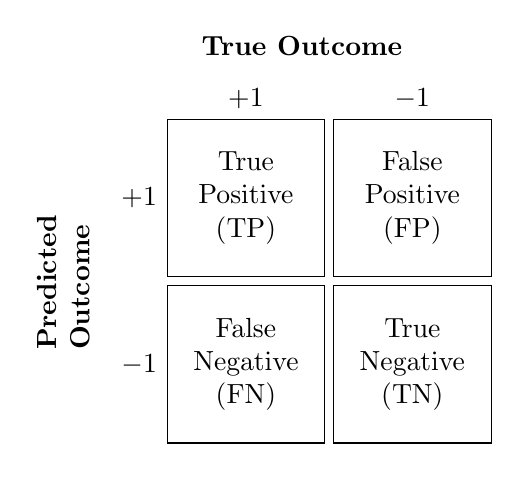
\begin{tikzpicture}[
    box/.style={draw,rectangle,minimum size=2cm,text width=1.5cm,align=center}]
    \matrix (conmat) [row sep=.1cm,column sep=.1cm] {
    \node (tpos) [box,
        label=left:$+1$,
        label=above:$+1$,
        ] {True \\ Positive (TP)};
    &
    \node (fneg) [box,
        label=above:$-1$,
        ] {False \\ Positive (FP)};
    \\
    \node (fpos) [box,
        label=left:$-1$,
        ] {False \\ Negative (FN)};
    &
    \node (tneg) [box,
        ] {True \\ Negative (TN)};
    \\
    };
    \node [rotate=90,left=0.5cm of conmat,text width=1cm,align=center] {\textbf{Predicted \\ Outcome}};
    \node [above =.05cm of conmat,align=center] {\textbf{True Outcome}};
    \end{tikzpicture}
    \caption{Confusion Matrix for binary classification task}
    \label{fig:confusion-matrix}
\end{figure}

\subsection{Receiver Operating Characteristics}
Now, the \textit{true positive rate} (TPR) is the measure of the number of correct positive predictions made out all the available true positive outcomes and is defined as, $TPR = TP/(TP+FN)$.
Similarly, the \textit{false positive rate} (FPR) measures the number of incorrect classifications of negative samples out of all the available negative samples, i.e., $FPR = FP/(FP+TN)$.
Therefore, the ROC curve is the space defined by the TPR as a function of the FPR, i.e., the TPR on y-axis and FPR on the x-axis. 
Each point on the ROC curve corresponds to a confusion matrix at some threshold.
A model that randomly predicts outcomes will plot a diagonal line, indicating that the TPR and FPR are equal.
A perfect classifier's plot would have a point at $(0,1)$, which indicates that there are no samples that are misclassified.
Although the ROC curve can be visually inspected to compare models, we utilize the \textit{area under the ROC curve} (AUC-ROC) as a quantitative measure of a model's performance.
Therefore, the baseline random model has a AUC-ROC of 0.5.

The AUC-ROC score is unaffected by an imbalanced dataset. 
This means that a high AUC-ROC score might hide the fact that the baseline accuracy of predicting all samples as positive might indeed be higher than 0.5.
Therefore, we need to be careful when interpreting the quality of the model solely based on the AUC-ROC score.

\subsection{Precision Recall}
\textit{Recall} is the same as true positive rate (TPR), i.e., $recall = TP/(TP+FN)$.
The ratio of the number of true positive predictions out of all the predicted positive outcomes is called \textit{precision} (or positive predictive rate).
It is defined as, $precision = TP/(TP+FP)$. 
Precision and recall are in tension, i.e., improving precision reduces recall and vice versa.
Therefore, the Precision-Recall (PR) curve is the space defined by representing precision as a function of recall, i.e., precision on y-axis and recall on the x-axis.
Each point on the PR curve corresponds to a single confusion matrix obtained from a particular value of the threshold $\theta$.
The baseline for the PR curve is based on the frequency of the positive label in the true outcomes and appears as a horizontal line in the plots.
Hence, the PR curve is affected by the imbalance present in the dataset.
Therefore, we define two measures to better represent the imbalances present in the \wikirfa dataset.

The PR curve is usually defined with respect to the positive label probability.
We refer to this curve as the positive PR curve and denote it by \posPR.
The positive baseline is computed as ratio of the true positive outputs and the total number of samples, $\text{baseline}_{\text{pos}} = (TP+FN)/(TP+FN+FP+TN)$.
This will be higher for the \wikirfa dataset as there are more positive samples, i.e., support votes.
We can measure the positive label performance by computing the area under the \posPR curve (\aucposPR), it is also called average precision score.
The \aucposPR score should be higher than the positive baseline to be significant.
Even so, the \aucposPR does not tell us if the model has learnt to predict negative votes equally well.

For this purpose, we define the negative PR curve as the PR curve where we consider the probability of predicting a negative outcome and denote it by \negPR.
As we have a binary classification task, if the positive probability vector is $\mathbf{p}$, then the negative probability vector is simply $\mathbf{1}-\mathbf{p}$.
Now considering $-1$ to be the positive label, we can plot a \negPR curve in the same manner.
The negative baseline for the \negPR curve is defined as the ratio of the true negative samples divided by the total number of samples, $\text{baseline}_{\text{neg}} = (TN+FP)/(TP+FN+FP+TN)$.
As the negative samples, i.e., oppose votes, are the minority in the \wikirfa dataset, the corresponding negative baseline will also be lower.
We can measure the performance of the model in predicting negative samples by computing the area under the \negPR curve (\aucnegPR).
This measure will be more important for evaluating the performance of the iterative models on the \wikirfa dataset.


\subsection{F1 Score}
The \textit{F1 score} is the harmonic mean of precision and recall and defined as 
\[
    F1 = 2\cdot\frac{\text{precision}\cdot\text{recall}}{\text{precision}+\text{recall}}.
\]
Therefore, if we consider a PR curve, then the F1 score is computed by taking the precision and recall values at a particular point on that curve.
If the curve was for the positive class probability, i.e., a \posPR curve, then we define the associated F1 score as the \posF score.
Similarly, if the curve is for the negative class probabilities, i.e., a \negPR curve, then the score is called the \negF score.
A simple average of the \posF and \negF scores is called the \textit{macro F1 score}, and is defined as follows,
\[ 
    \text{F1}_{\text{macro}} = \frac{\text{F1}_{\text{pos}}+\text{F1}_{\text{neg}}}{2}.
\]
The \macroF score is useful for datasets which are imbalanced as it places equal weight on the performance for both positive and negative labels.

All the metrics in the previous subsubsection used probabilities directly to evaluate the overall performance of the model.
As the F1 score is calculated for a point in the PR curve, it corresponds to the particular value of threshold $\theta$, that yielded those values of precision and recall in the confusion matrix.
Therefore, we can now plot the F1 score as a function of the threshold. 
This allows us to analyse both the \posF and \negF plots versus the threshold and choose the optimal value of $\theta$, that maximizes the \macroF score.
Hence, we can understand how the model will perform when asked to deterministically predict classes.



% \chapter{Evaluation}
\label{chapter:evaluation}

You have done your work, but that's\footnote{By the way, do \emph{not} use
shorthands like this in your text! It is not professional! Always write out all
the words: ``that is''.} not enough. 

You also need to evaluate how well your implementation works.  The
nature of the evaluation depends on your problem, your method, and
your implementation that are all described in the thesis before this
chapter.  If you have created a program for exact-text matching, then
you measure how long it takes for your implementation to search for
different patterns, and compare it against the implementation that was
used before.  If you have designed a process for managing software
projects, you perhaps interview people working with a waterfall-style
management process, have them adapt your management process, and
interview them again after they have worked with your process for some
time. See what's changed.

The important thing is that you can evaluate your success somehow.
Remember that you do not have to succeed in making something spectacular; a
total implementation failure may still give grounds for a very good master's
thesis---if you can analyze what went wrong and what should have been
done. 

 

 
% \chapter{Discussion}
\label{chapter:discussion}

At this point, you will have some insightful thoughts on your
implementation and you may have ideas on what could be done in the
future. This chapter may be combined together with the evaluation
chapter. All the new insights and findings are given here!  This
chapter is a good place to discuss your thesis as a whole and to show
your professor that you have really understood some non-trivial
aspects of the methods you used\ldots


 
% \chapter{Conclusions}
\label{chapter:conclusions}

Time to wrap it up!  Write down the most important findings from your
work.  Like the introduction, this chapter is not very long.  One to
two (never over three) pages might be a good limit. Still, the chapter
gives the background, goals, content, and the findings. However, all that
should already be in the previous chapters. This is just a summary (as
are the abstract and the introduction).

For making PDF/A version requested by the Aalto Library, open the end result pdf file in Acrobat and store it as PDF/A. Then verify the result (everything should be fine, at least as PDF/A-2b version works).

Congratulations, your thesis is ready and it looks beautiful!



% Load the bibliographic references
% ------------------------------------------------------------------
% You can use several .bib files:
% \bibliography{thesis_sources,ietf_sources}
\bibliography{sources}


% Appendices go here
% ------------------------------------------------------------------
% If you do not have appendices, comment out the following lines

% \appendix
% \chapter{First appendix}
\label{chapter:first-appendix}

This is the first appendix. You could put some test images or verbose data in an
appendix, if there is too much data to fit in the actual text nicely.

For now, the Aalto logo variants are shown in Figure~\ref{fig:aaltologo}.

\begin{figure}
\begin{center}
\subfigure[In English]{
\includegraphics[width=.8\textwidth]{images/aalto-logo-en}}
\subfigure[Suomeksi]{
\includegraphics[width=.8\textwidth]{images/aalto-logo-fi}}
\subfigure[P� svenska]{
\includegraphics[width=.8\textwidth]{images/aalto-logo-se}}
\caption{Aalto logo variants}
\label{fig:aaltologo}
\end{center}
\end{figure}


% End of document!
% ------------------------------------------------------------------
% The LastPage package automatically places a label on the last page.
% That works better than placing a label here manually, because the
% label might not go to the actual last page, if LaTeX needs to place
% floats (that is, figures, tables, and such) to the end of the 
% document.
\end{document}